\documentclass[journal]{IEEEtran}

\usepackage{graphicx}
\usepackage{amsmath,amssymb}
\usepackage{textcomp}
\usepackage{url}
\usepackage{array}
\usepackage{booktabs}
\usepackage{adjustbox}
\usepackage{tabularx}

\graphicspath{{figs/}}

\begin{document}

\title{Building the Cities of Tomorrow: Technology, Infrastructure, and Sustainability}

\author{Jaishnu~Sree~Biradha, Suseela~Sellamuthu, Bhavadharini~R.~M., Krithiga~R., and Vedhapriyavadhana~Rajamani%
\thanks{J. S. Biradha, S. Sellamuthu, B. R. M., and K. R. are with the School of Computer Science and Engineering (SCOPE), Vellore Institute of Technology, Chennai, Tamil Nadu, India (e-mail: suseela.s@vit.ac.in).}%
\thanks{V. Rajamani is with the School of Computing, Engineering and Physical Sciences, University of the West of Scotland, London, U.K. (e-mail: vedhapriyavadhana.rajamani@uws.ac.uk).}%
\thanks{Corresponding author: Suseela Sellamuthu (e-mail: suseela.s@vit.ac.in).}%
}

\markboth{Smart Cities Review}{Biradha \emph{et al.}: Building the Cities of Tomorrow: Technology, Infrastructure, and Sustainability}

\maketitle

\begin{abstract}
Smart cities represent an innovative approach to urban development that combines data-driven technologies with sophisticated management practices to raise residents' quality of life, strengthen sustainability, and stimulate economic growth. This review surveys the principal innovations and technologies that drive smart city development, including the Internet of Things (IoT), artificial intelligence (AI), big data analytics, and renewable energy systems, and examines the infrastructure components -- smart transportation, energy-efficient buildings, modern waste treatment, and reliable connectivity -- on which these efforts depend. Drawing on case studies from Singapore, Barcelona, Dubai, New York City, and other leading urban centers, the paper distills practical lessons and best practices from real-world deployments. It further examines the international partnerships, multilateral initiatives, and interoperability standards that enable smart city programs to scale and interconnect across borders. The findings are synthesized into a strategic roadmap for future smart city development, one that depends on sustained stakeholder collaboration, robust policy frameworks, and long-term planning to address the challenges that lie ahead.
\end{abstract}

\begin{IEEEkeywords}
Artificial Intelligence (AI), Digital Infrastructure, Global Collaboration, Internet of Things (IoT), Smart Cities, Sustainability
\end{IEEEkeywords}

\section{Introduction}
The smart city has emerged as the defining model of urban life in the twenty-first century, shaped by decades of technological progress and innovation. At its core, a smart city relies on Information and Communication Technologies (ICT) to raise the quality of life of its residents by improving the delivery of essential services, including smart healthcare, smart mobility, smart retail, smart homes, education, and smart energy and transport systems, as illustrated in Fig.~\ref{fig:services}.

\begin{figure}[ht]
\centering
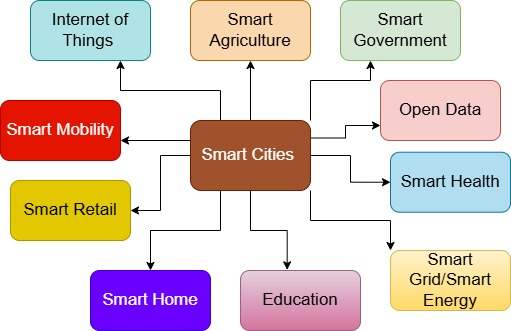
\includegraphics[width=\linewidth]{image-001.jpeg}
\caption{Smart Cities Services}
\label{fig:services}
\end{figure}

By embedding digital technologies into city infrastructure, smart cities can lower resource consumption, sharpen decision-making, and deepen citizen engagement. Smart city development is not simply a matter of installing new hardware; it is the construction of interconnected ecosystems that use data-driven solutions to confront the mounting pressures of urbanization -- traffic congestion, pollution, and resource scarcity chief among them \cite{r1,r5}. Fig.~\ref{fig:framework} depicts how a smart city is built from a constellation of IoT devices, sensors, and cloud-based platforms that work together to capture and process information in real time.

\begin{figure}[ht]
\centering
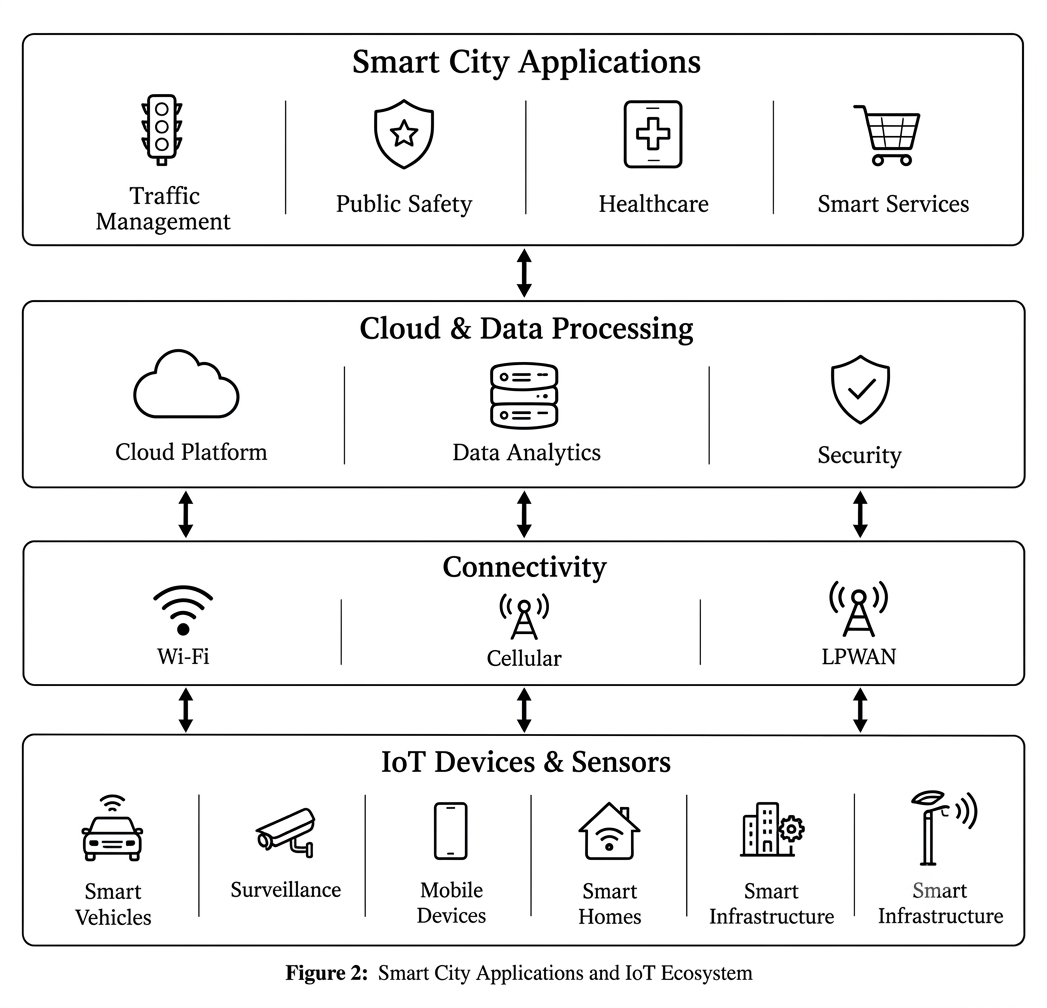
\includegraphics[width=\linewidth]{image-002.png}
\caption{Smart City Framework}
\label{fig:framework}
\end{figure}

This real-time information base allows city administrations to make better-informed decisions, whether in optimizing traffic flow, regulating energy distribution, or improving public safety \cite{r1}. Road-monitoring systems, for example, assess pavement and traffic conditions and adjust signal timing accordingly, reducing congestion and emissions \cite{r3}. Smart grids allocate electricity more efficiently, cutting waste and directing power to where it is most needed. Beyond raising operational efficiency, such technologies help cities meet sustainability targets that become more pressing as urban populations continue to grow \cite{r4}. Shao and Min catalog a broad range of sustainability measures relevant to smart city development \cite{r107}, while noting that multidimensional sustainability models remain largely confined to conceptual frameworks rather than operational practice. Singh \emph{et al.} take a wider historical view, tracing a decade of technological advances, architectural models, and platforms in smart city research \cite{r108}; their methodological survey of sensing technologies, communication layers, data management, and application domains lays a solid technical foundation for the study of smart urban development, while also flagging governance integration, citizen engagement, global interoperability, and cross-case comparison as areas that warrant further attention. Han and Kim likewise identify a persistent gap between technology-oriented research and the realities of urban environments, governance structures, infrastructure integration, and international benchmarking \cite{r7}.

Despite the substantial body of literature on smart cities, several important areas remain underexplored. This review addresses the innovation, technology, and infrastructure dimensions of smart city development in a globalized context, while also considering smart governance, inclusiveness, international standards, and comparative examples drawn from leading cities such as Singapore, Barcelona, Dubai, and New York City. It systematically links technological innovation with physical and virtual infrastructure, governance structures, citizen participation, and sustainability goals, and offers a perspective on data privacy, social equity, and regulatory policy that seeks to close the fragmentation and contextual gaps evident in the existing literature.

As smart technologies spread across the globe, collaboration and standardization have become increasingly central to their success. Cities are turning to international standards, partnerships, and city networks to share best practices, data, and resources, and to build the interoperability that connects individually smart cities into a genuinely global movement. Singapore, Barcelona, Dubai, and New York City stand out as exemplars of both urban innovation and international collaboration \cite{r8}. At the same time, the challenges facing smart cities -- data privacy, security, inclusivity, and the need for resilient policy frameworks -- have grown in step with their capabilities, since the same technologies that unlock efficiency also increase the volume of data that must be managed responsibly and the difficulty of ensuring equitable access to their benefits \cite{r9,r101}.

This review is intended for policymakers, researchers, and industry practitioners in both developed and developing countries who seek to understand how smart cities are evolving, the obstacles they face, and the direction they must take to become more interconnected, resilient, and inclusive. It analyzes how innovation, technology, and infrastructure can be combined to transform urban life, and argues that international cooperation is indispensable to accelerating the adoption of these benefits across world-leading cities such as Singapore, Barcelona, Dubai, and New York City, among others \cite{r12,r13}.

\begin{figure}[ht]
\centering
\begin{tabular}{@{}c@{}}
\textbf{1. Introduction}\\
\textbf{2. Smart City Infrastructure}\\
\qquad 2.1 Digital Infrastructure\\
\qquad 2.2 Physical Infrastructure\\
\qquad 2.3 Urban Planning and Design\\
\textbf{3. Innovation and Technology in Smart Cities}\\
\textbf{4. Global Connectivity in Smart Cities}\\
\qquad 4.1 Standards and Interoperability\\
\qquad 4.2 International Collaboration\\
\textbf{5. Sustainability and Smart Cities}\\
\qquad 5.1 Role of SDGs\\
\qquad 5.2 Country-Level Initiatives\\
\qquad 5.3 Case Studies (India, Singapore, EU, UAE, USA)\\
\textbf{6. Challenges and Future Directions}\\
\textbf{7. Conclusion}\\
\textbf{8. References}
\end{tabular}
\caption{Glimpse of Review Paper}
\label{fig:outline}
\end{figure}

The remainder of this paper is organized as shown in Fig.~\ref{fig:outline}. Section II examines smart city infrastructure; Section III discusses innovation and technology; Section IV addresses global connectivity among smart cities; Section V explores the role of the Sustainable Development Goals (SDGs); and Section VI discusses the challenges and future directions facing the field. Section VII concludes the paper.

\section{Smart City Infrastructure}
Urbanization and population growth have intensified demand for efficient and sustainable city management, and infrastructure sits at the heart of how smart cities are built and operated. Smart city infrastructure blends conventional municipal facilities with digital technologies to sharpen the efficiency of public services, resource management, and communication networks, and thereby helps deliver smart solutions that raise citizens' quality of life while supporting sustainable urban development. Well-integrated infrastructure is consequently a precondition for successful smart city implementation. This section organizes infrastructure into three categories -- digital infrastructure, physical infrastructure, and urban planning and design -- as depicted in Fig.~\ref{fig:infrastructure}.

\begin{figure}[ht]
\centering
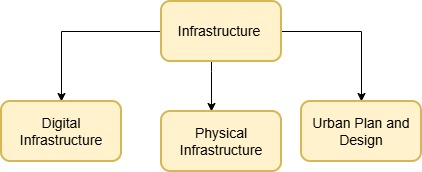
\includegraphics[width=\linewidth]{image-003.jpeg}
\caption{Smart City Infrastructure}
\label{fig:infrastructure}
\end{figure}

\subsection{Digital Infrastructure in Smart Cities}
Urban infrastructure has evolved considerably over the centuries. Preindustrial cities concentrated on basic amenities such as roads, water supply, and waste disposal. The Industrial Revolution introduced major innovations -- railways, electrical networks, and telecommunications systems -- and digital infrastructure followed with the advent of the internet and digital technologies toward the end of the twentieth century. Contemporary urban challenges have, in turn, driven the integration of smart city infrastructure with these earlier digital layers.

Digital infrastructure is the basic building block of smart city development: it enables communication, data transfer, and connectivity among the city's various systems by combining information and communication technologies (ICT), sensor networks, cloud platforms, and data centers to support effective management and real-time decision-making, as shown in Fig.~\ref{fig:components}. This infrastructure stores, collects, processes, and transfers data across the city, and comprises IoT sensors and devices, a communication network layer, edge computing, cloud computing, and smart city applications.

\begin{figure}[ht]
\centering
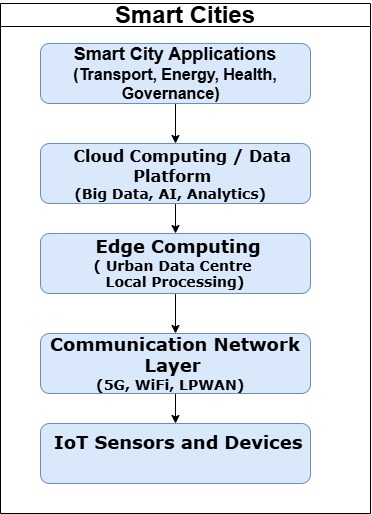
\includegraphics[width=0.72\linewidth]{image-004.jpeg}
\caption{Components of Smart Cities}
\label{fig:components}
\end{figure}

Digital infrastructure allows smart cities to strengthen service delivery and operational effectiveness while extending connectivity to citizens. It underpins the latest generation of urban technologies aimed at improving city life, managing resources, and enhancing service quality, and is turning cities into platforms capable of real-time monitoring, data-driven decision-making, and reliably functioning urban systems. Investment in this infrastructure continues to grow, and studies have documented the substantial economic returns generated by smart city investment \cite{r102}.

\subsubsection{Components of Digital Infrastructure}
Fig.~\ref{fig:components} illustrates how the interconnected components of digital infrastructure collectively enable a seamless flow of data and information. IoT sensors collect real-time data from the physical environment, while data centers store and process it; urban data centers, in particular, specialize in collecting and analyzing urban data. Cloud computing supplies scalable, on-demand computing resources, and the combination of these elements -- unified by a framework of technologies, protocols, and standards -- supports effective communication and data exchange. This connected ecosystem underlies the growing range of applications and services that drive innovation across an increasingly digitalized world.

IoT sensors gather information on numerous variables, including temperature, humidity, air quality, traffic flow, and energy consumption. Distributed throughout the city, these sensors supply the real-time data needed to monitor and control municipal systems. A smart traffic light exemplifies this process: linked to IoT sensors, it adjusts signal timing according to current traffic conditions to reduce congestion and emissions. IoT applications across transportation, energy, and infrastructure management generate substantial economic value for cities \cite{r15}.

Realizing this potential requires a holistic strategy encompassing sensor selection and deployment, effective data collection and transmission, accurate data analysis and processing, complete interconnection with existing city systems, and rigorous attention to security, privacy, and ethics. Cities that implement such strategies effectively are positioned to unlock the full potential of IoT and, in turn, become smarter, more resilient, and more sustainable \cite{r15}.

Rapid advances in IoT technology have become central to making cities smarter, since IoT supplies the technological foundation on which innovative, automated, and interoperable services and applications are built across urban contexts. Data centers -- facilities that house computing, storage, and networking equipment -- provide the computational capacity needed to process and store the large volumes of data that IoT devices generate. Modern data centers are built around the principles of virtualization and containerization, which optimize resource use and maximize uptime, making them a central component in the effective processing and analysis of city data. \textbf{Data centers thus form the backbone of smart city operations, providing the scalable computing and storage capacity required to process and analyze the large volumes of data generated by city systems \cite{r16}.}

Cloud computing supplies scalable, flexible computing resources over the internet, allowing cities to deploy and operate smart city applications without heavy up-front investment in physical hardware. Cloud platforms offer data storage, analytics, and machine learning services that are essential to developing and running smart city solutions; for instance, cloud computing can aggregate and analyze data from disparate sources to generate actionable insight for city officials. The growing reliance of smart city operations on cloud platforms for storage, analytics, and machine learning reflects the deepening integration of cloud computing with the Internet of Things in urban environments \cite{r10}.

Urban data platforms are centralized systems that combine information drawn from IoT devices, social media, and open databases. These platforms enable data sharing and collaboration across city departments and stakeholders, supporting integrated city management, while data visualization and analysis tools help decision-makers translate raw data into policy action. An urban data platform might, for example, integrate traffic, weather, and transport data to streamline urban mobility.

\subsubsection{Impacts of Digital Infrastructure}
Digital infrastructure is reshaping urban mobility by adapting new technologies to streamline transport networks. Recent work on integrated ICT-based service delivery models for smart mobility shows how such models can enhance sustainability, mobility performance, and quality of life in city centers \cite{r107,r15}. IoT sensors and data analytics support effective traffic control, cutting congestion and travel time, while real-time coordination of public transport schedules and availability improves the efficiency and reliability of transit systems. Smart parking is a representative example: IoT sensors provide real-time updates on space availability, saving drivers time and reducing the emissions generated by vehicles idling while searching for parking. Smart traffic management systems have been shown to improve transportation performance, enhance travel safety, and reduce congestion, generating substantial economic benefits for cities \cite{r12}.

Digital infrastructure also strengthens public safety through advanced surveillance and data-driven response. Facial-recognition and video-analytics systems support real-time monitoring and rapid incident response, sharpening situational awareness, while IoT sensors such as gunshot detectors can alert police to potential threats before they escalate. Intelligent street lighting further deters crime by adjusting illumination dynamically according to activity levels in an area \cite{r13,r17}. New York City's Domain Awareness System illustrates this approach at scale, drawing on more than 9,000 cameras to give police real-time intelligence; the system has played a significant role in reducing crime by enabling faster, better-informed decisions during critical incidents \cite{r14,r18}.

Digital infrastructure enables smart energy management by monitoring and controlling energy use within buildings and public infrastructure. Research on IoT-based energy management systems in smart buildings and urban infrastructure shows that such systems facilitate the collection and analysis of data needed to monitor, control, and optimize energy use, thereby lowering environmental impact while improving efficiency and sustainability \cite{r108,r19}.

Smart grids use IoT sensors to balance energy supply and demand, reducing waste and improving efficiency, while smart meters give consumers real-time visibility into their energy consumption and encourage more efficient use. Cities can use the data from smart meters to implement dynamic pricing that shifts consumption toward off-peak hours. Smart grids equipped with advanced sensing and communication technologies can substantially reduce transmission and distribution losses, which matters for the energy-intensive applications and services that smart cities depend on \cite{r98}.

Satellite broadband extends internet access to remote or rural regions where terrestrial broadband is unavailable. Although capable of speeds up to 100 Mbps, satellite broadband typically carries higher latency due to the long distances signals must travel to and from orbit; even so, satellite services continue to expand as a complement to terrestrial networks, helping to close connectivity gaps in remote and underserved areas \cite{r20,r21}.

Fourth-generation LTE and 5G networks exemplify wireless broadband, delivering high-speed internet without the constraints of physical cabling and offering flexibility and scalability that wired networks cannot match. Wireless broadband is essential for mobile connectivity and for extending internet access to locations where traditional infrastructure is difficult to deploy, and its role is expected to grow further as 5G networks expand and smart city applications demand ever greater capacity \cite{r22}.

Smart homes and buildings rely on high-speed broadband to connect and manage IoT devices, security systems, and smart appliances, giving residents remote control over energy use, security, and home environments. Reliable high-speed connectivity is therefore a prerequisite for these remote monitoring and control functions \cite{r23}.

Smart transportation systems likewise depend on high-speed broadband, which connects self-driving vehicles, smart streetlights, and real-time transportation systems, improving traffic flow and reducing congestion. Since human error is responsible for the majority of road accidents, connected and automated driving technologies enabled by broadband connectivity offer a path to safer transportation systems \cite{r24}.

High-speed broadband also enables efficient online delivery of government services, increasing transparency while lowering administrative costs; citizens can make payments and conduct civic business from home rather than visiting a government office in person. Countries with more developed broadband infrastructure tend to post higher e-government development index (EGDI) scores, reflecting more efficient access to electronic government services \cite{r25}.

In education, high-speed broadband has become essential to e-learning for both students and teachers, providing access to online resources, virtual classrooms, and collaboration tools, and supporting education platforms that reach learners regardless of location. The COVID-19 pandemic underscored this dependency: as school closures forced a rapid shift to online learning, broadband-enabled platforms became, for many students worldwide, the only available means of continuing their education \cite{r26}.

Seoul, South Korea, has deployed a fast, extensive broadband network that supports gigabit internet and a wide range of smart city applications, including smart transportation, community safety initiatives, and e-governance services \cite{r27}. Stockholm has similarly deployed a municipally owned fiber network that delivers high-speed access to nearly every household and business in the city, supporting smart grids, intelligent transport, and sustainable urban development \cite{r28}.

Enhanced broadband infrastructure carries substantial economic benefits and raises living standards: faster internet access supports business and productivity, fuels innovation, and improves access to education, healthcare, and public services. Empirical research on OECD countries has found that a ten-percentage-point increase in broadband penetration raises annual per-capita GDP growth by roughly one percentage point \cite{r29}.

Broadband infrastructure nonetheless faces significant challenges. High deployment costs -- driven by cable installation, equipment, and maintenance -- make such projects difficult to finance in low-resource areas, while geographic and demographic disparities leave many rural and remote regions without adequate infrastructure, widening the digital divide; access to high-speed internet also continues to depend on socioeconomic factors. Studies in the United States have documented a persistent gap in broadband access and adoption between metropolitan and non-metropolitan areas \cite{r31}.

The same connectivity that enables smart city services also exposes them to threats and vulnerabilities: data breaches, cyberattacks, and malware can disrupt services and compromise sensitive information, underscoring the critical importance of cybersecurity to the protection of digital infrastructure. Regulatory hurdles -- including cumbersome permitting procedures, spectrum allocation challenges, and inconsistent regulation across regions -- further complicate broadband deployment; streamlining permitting processes and coordinating spectrum policy are widely viewed as important levers for encouraging investment in broadband infrastructure \cite{r30}.

\subsubsection{Technological Advancements}
Gigabit Ethernet over fiber-optic networks supports data-transfer rates of 1 Gbps or higher and forms a significant component of high-speed broadband networks, delivering fast, reliable connectivity for homes and businesses and underpinning many wireless broadband services as well. Governed by the IEEE 802.3 standard, Gigabit Ethernet has evolved to support higher-speed variants -- 10 Gbps, 40 Gbps, and 100 Gbps -- that accommodate growing data-transfer demands.

Wi-Fi 6 (802.11ax) improves substantially on earlier generations of Wi-Fi, supporting speeds up to 9.6 Gbps and handling a far greater number of simultaneous connections, which makes it well suited to smart homes and high-density urban environments. Mesh networks complement this capability by providing continuous Wi-Fi coverage through a web of interconnected nodes.

Continued innovation in broadband technology -- higher-capacity fiber-optic cables, improved transmission methods, and emerging approaches such as Li-Fi, which transmits data using light, and quantum communication, which promises ultra-secure data transfer -- will further extend broadband capability. Researchers at the University of California, Santa Barbara, for example, are investigating how photonic integrated circuits can improve the performance and scalability of fiber-optic networks \cite{r33}.

Fifth-generation (5G) networks represent a substantial improvement over earlier generations, offering faster speeds, lower latency, and greater capacity through advanced technologies such as millimeter waves, small cells, massive MIMO (multiple-input multiple-output), and beamforming. 5G networks are designed to support up to one million connected devices per square kilometer, peak data rates of up to 20 Gbps, and latencies as low as one millisecond, making 5G up to 100 times faster than 4G and enabling rapid streaming, data transfer, and high-definition video calling. This low latency supports the real-time communication essential to applications such as autonomous vehicles and remote surgery, and 5G's greater device density is vital to the IoT deployments that smart cities depend on \cite{r36}.

5G infrastructure supplies the real-time communication and IoT connectivity platform on which smart city applications are built \cite{r36}, serving as a driver of applications that make city life more efficient, sustainable, and livable, and integrating readily with healthcare, public safety, energy management, and transportation systems.

5G operates across three frequency bands: low-band (sub-1 GHz), mid-band (1--6 GHz), and high-band (24--100 GHz, millimeter wave). Low-band offers greater coverage and building penetration, making it well suited to rural and suburban areas; mid-band serves urban areas with moderate-to-high data demands; and high-band delivers very high speeds and capacity but only over the short ranges and limited penetration typical of dense urban areas and specific high-demand applications \cite{r37}.

Cellular radio access networks operate at low power over smaller coverage radii, delivering greater network capacity, particularly in high-density urban locations. MIMO, beamforming, and network slicing are the principal technologies used to improve the quality of smart networks. Multiple-input multiple-output (MIMO) is a wireless technology that uses multiple antennas at both transmitter and receiver to send and receive more data simultaneously, supporting the high data traffic generated by IoT devices; MIMO underlies surveillance cameras, smart traffic systems, and public Wi-Fi networks.

Beamforming, used across MIMO and 5G systems, directs signals toward a specific user or device rather than broadcasting in all directions, reducing interference, ensuring high-speed data transfer, and supporting large numbers of simultaneous IoT connections.

Network slicing is a key 5G technology that divides a single physical network into multiple virtual networks, or slices, each tailored to a specific service or application to guarantee performance, reliability, and effectiveness. In smart cities, network slicing creates multiple virtual networks within a single physical infrastructure, with each slice optimized for applications such as smart transportation, public safety and emergency services, and smart surveillance \cite{r38}. Table~\ref{tab:slicing} summarizes representative use cases of network slicing.

\begin{table}[!t]
\caption{Use Cases of Network Slicing}
\label{tab:slicing}
\centering
\begin{tabular}{@{}p{0.32\linewidth}p{0.63\linewidth}@{}}
\toprule
\textbf{Use Case} & \textbf{Description}\\
\midrule
Smart Transportation & Operates with ultra-low latency. Dedicated slice for traffic control and autonomous vehicles, providing the real-time data processing needed to ensure safety and faster transportation\\
Public Safety \& Emergency Services & Separate slice for police, fire, and ambulance services. Ensures reliable communication even during network congestion\\
Smart Surveillance & High-bandwidth slice for CCTV cameras and AI-based video analytics. Enables real-time monitoring and crime prevention\\
\bottomrule
\end{tabular}
\end{table}

Mobile broadband powered by 5G gives people, businesses, and government services a faster, more secure internet connection, enabling high-definition video streaming, augmented and virtual reality, and other data-intensive applications that raise living standards in cities. The widespread adoption of 5G is expected to drive significant growth in mobile data traffic and network capacity \cite{r36}.

Ultra-Reliable Low-Latency Communication (URLLC), another key 5G feature, enables the real-time communication required by services such as autonomous driving, industrial automation, and remote healthcare, where low latency and high reliability are essential to safety and accuracy. 5G-enabled URLLC combined with enhanced vehicle-to-everything (V2X) communication is a key enabler of safety-critical road traffic applications \cite{r36}.

Massive Machine-Type Communications (mMTC), a further 5G feature, connects several thousand IoT devices in scenarios that demand frequent but low-rate transmissions, and is designed to support extremely large numbers of connected devices, such as smart meters, environmental sensors, and connected streetlights across smart city infrastructure \cite{r36}.

Taken together, 5G promises to transform high-speed broadband systems through much greater speed, lower latency, and wider connectivity, enabling a wide range of applications spanning the IoT, self-driving vehicles, and augmented reality. As 5G networks are deployed, smart cities will gain the capacity to share data in real time and deliver increasingly sophisticated services.

Extending digital access to rural regions and underserved communities remains a policy priority. Governments and private-sector partners are investing in subsidies, grants, and public--private partnerships to close the digital divide, while emerging technologies such as low-Earth-orbit (LEO) satellites promise to bring high-speed internet to remote locations. In the United States, the Rural Digital Opportunity Fund (RDOF) is subsidizing broadband deployment in unserved areas with billions of dollars in funding \cite{r32}.

\subsubsection{5G in Smart Cities}
Fifth-generation mobile networks underpin smart city development by delivering low latency, ultra-fast speed, and massive connectivity for millions of devices. 5G supports smart transport systems that exchange real-time information among infrastructure, vehicles, and traffic management systems, as depicted in Fig.~\ref{fig:5g-transport}, enabling automated driving, adaptive traffic signals, and flexible route mapping that together improve the flow and safety of traffic.

\begin{figure}[ht]
\centering
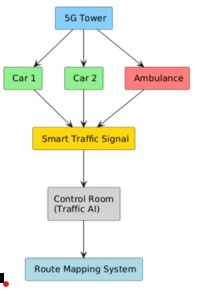
\includegraphics[width=0.72\linewidth]{image-005.jpeg}
\caption{5G-enabled Smart Transportation Systems}
\label{fig:5g-transport}
\end{figure}

\begin{figure}[ht]
\centering
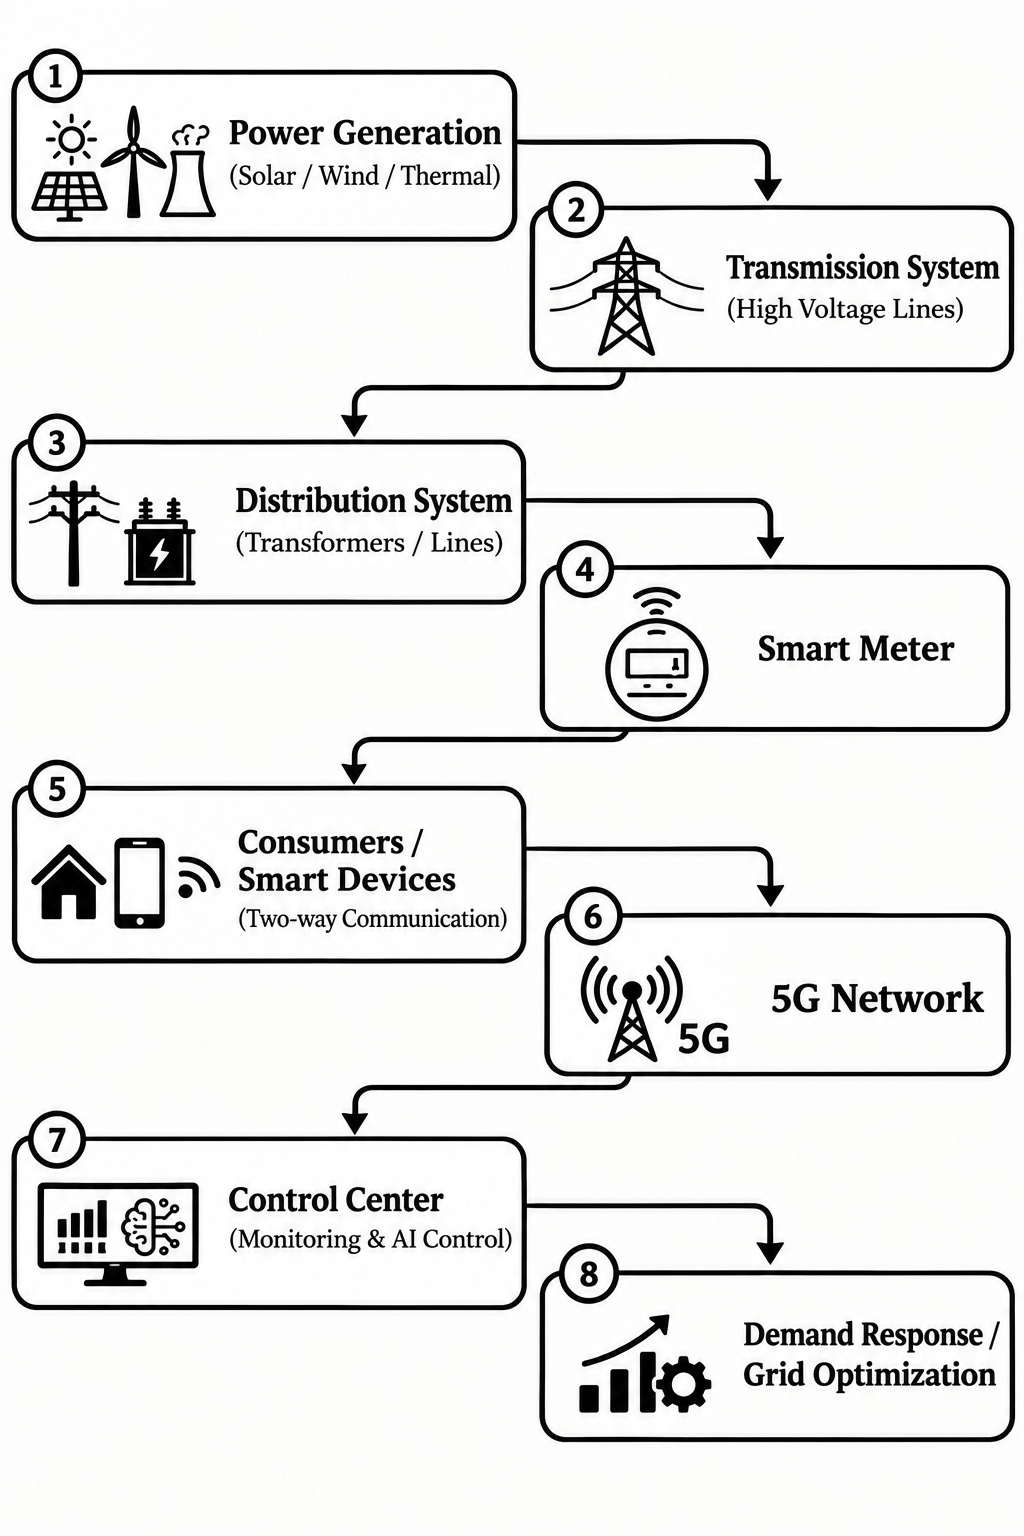
\includegraphics[width=0.72\linewidth]{image-006.png}
\caption{5G Network Connectivity in Smart Cities}
\label{fig:5g-connectivity}
\end{figure}

\begin{figure}[ht]
\centering
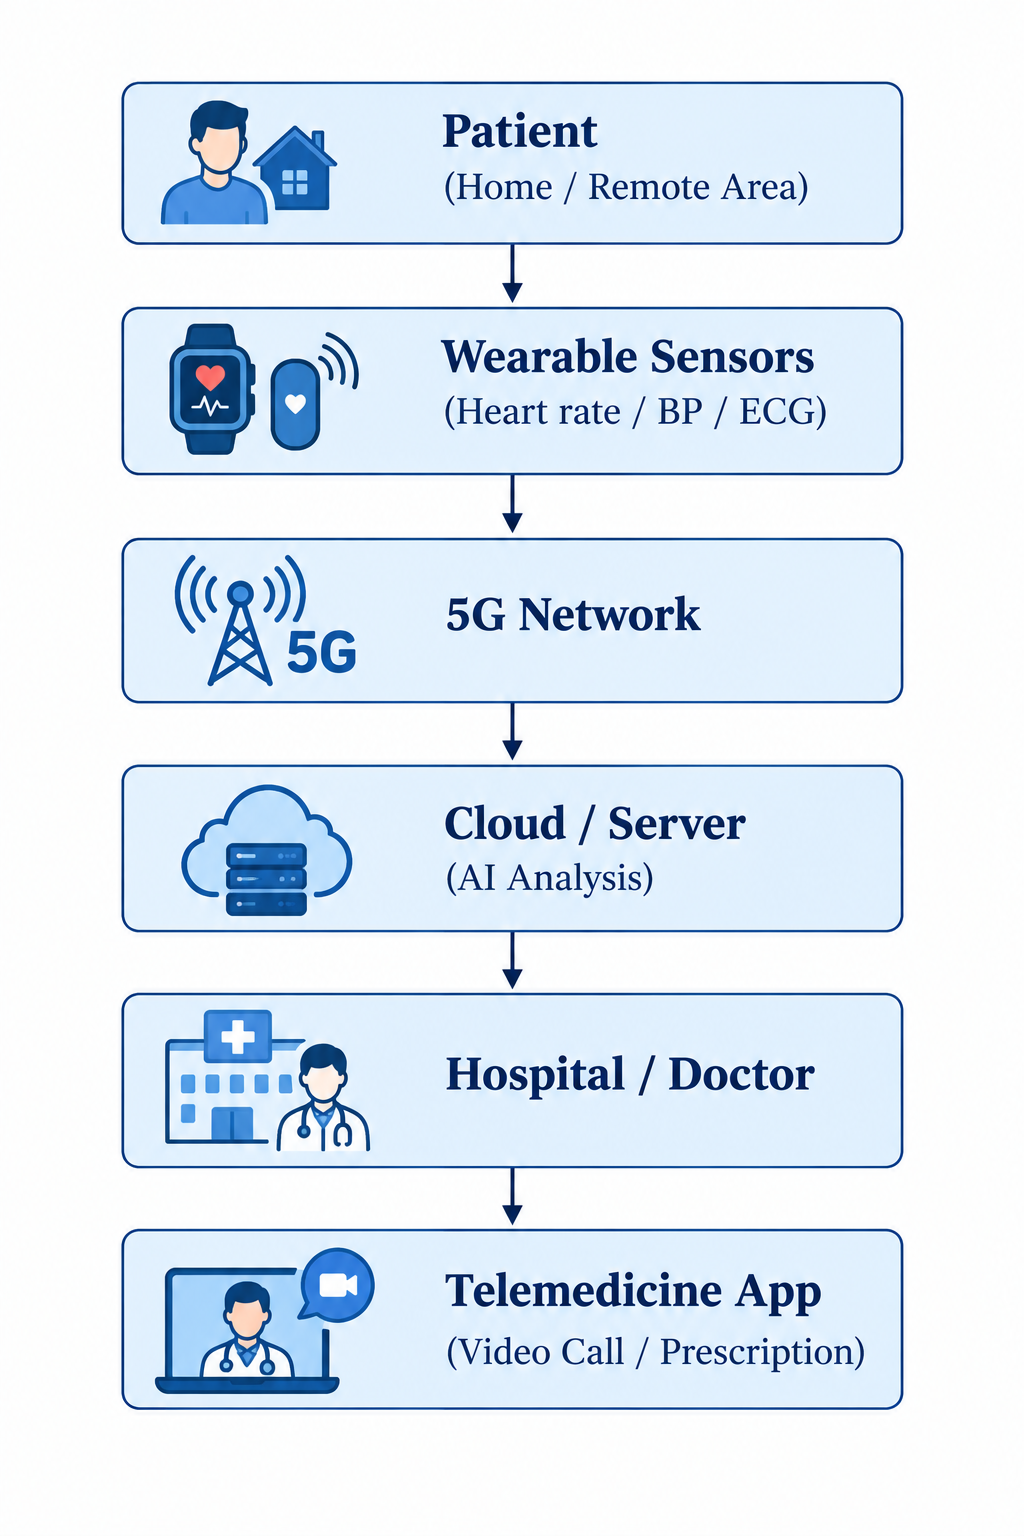
\includegraphics[width=0.72\linewidth]{image-007.png}
\caption{5G-enabled Vehicle-to-Everything (V2X) Communication}
\label{fig:5g-v2x}
\end{figure}

Vehicle-to-everything (V2X) technologies allow connected and automated vehicles to communicate with one another and with roadside infrastructure. The high reliability and low latency of 5G networks are essential to supporting this communication and helping autonomous vehicles operate safely and efficiently \cite{r43}.

Smart grids paired with 5G enable real-time monitoring and control of energy systems: smart grid communication technologies support efficient energy distribution, integration of renewable power sources, and rapid response to shifts in demand, making urban energy systems more sustainable and reliable \cite{r44}. Fig.~\ref{fig:5g-grid} illustrates the architecture of a 5G-enabled smart grid.

\begin{figure}[ht]
\centering
\begin{tabular}{@{}c@{}}
{\textbf{Power Generation}}\\
(Solar / Wind / Thermal)\\
$\downarrow$\\
{\textbf{Transmission System}}\\
(High Voltage Lines)\\
$\downarrow$\\
{\textbf{Distribution System}}\\
(Transformers / Lines)\\
$\downarrow$\\
{\textbf{Smart Meter}}\\
$\downarrow$\\
{\textbf{Consumers / Smart Devices}}\\
$\uparrow$\\
(Two-way Communication)\\
$\downarrow$\\
\textbf{5G Network}\\
$\downarrow$\\
{\textbf{Control Center}}\\
(Monitoring \& AI Control)\\
$\downarrow$\\
{\textbf{Demand Response / Grid Optimization}}
\end{tabular}
\caption{5G-enabled Smart Grid Architecture}
\label{fig:5g-grid}
\end{figure}

5G also strengthens public safety by enabling real-time communication and coordination among emergency responders, supporting applications such as remote monitoring, predictive data analysis, and rapid resource mobilization that allow cities to respond to emergencies faster and more effectively. Research on public safety communications shows that 5G capabilities can transform emergency response by giving first responders better situational awareness and coordination \cite{r45}, although deployment remains most demanding in densely populated urban centers and areas with limited existing infrastructure. Fig.~\ref{fig:5g-safety} shows a representative 5G-based emergency-response framework.

\begin{figure*}[!t]
\centering
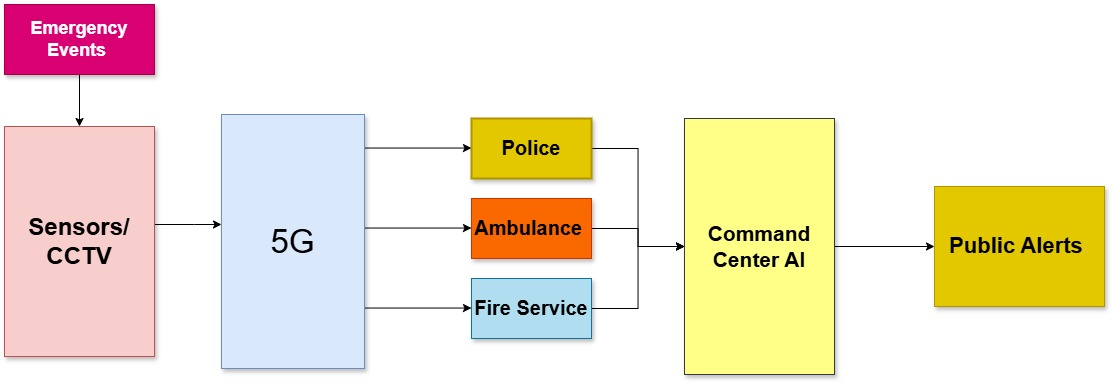
\includegraphics[width=\textwidth]{image-008.jpeg}
\caption{5G for Public Safety and Emergency Response}
\label{fig:5g-safety}
\end{figure*}

5G is also transforming healthcare by enabling telemedicine, remote patient monitoring, and more sophisticated medical procedures. High-definition video consultation, real-time transmission of medical data, and remote-assisted procedures together make healthcare services more efficient and more widely accessible, improving patient outcomes as a result. Fig.~\ref{fig:5g-health} depicts a representative 5G-enabled remote healthcare workflow.

\begin{figure}[ht]
\centering
\begin{tabular}{@{}c@{}}
{\textbf{Patient}} (Home / Remote Area)\\
$\downarrow$\\
{\textbf{Wearable Sensors}}\\
(Heart rate / BP / ECG)\\
$\downarrow$\\
\textbf{5G Network}\\
$\downarrow$\\
{\textbf{Cloud / Server}} (AI Analysis)\\
$\downarrow$\\
{\textbf{Hospital / Doctor}}\\
$\downarrow$\\
{\textbf{Telemedicine App}}\\
(Video Call / Prescription)
\end{tabular}
\caption{5G-enabled Remote Healthcare}
\label{fig:5g-health}
\end{figure}

5G is a similarly important enabler of Industry 4.0 in smart manufacturing, supporting interconnected factories and automated, real-time data analytics that draw on IoT, robotics, and artificial intelligence to improve production, flexibility, and quality. By enabling real-time data exchange and automation across the production chain, 5G supports productivity gains in smart manufacturing and industrial automation \cite{r97}. Fig.~\ref{fig:manufacturing} depicts the overall data and material flow in a 5G-enabled smart factory.

\begin{figure}[ht]
\centering
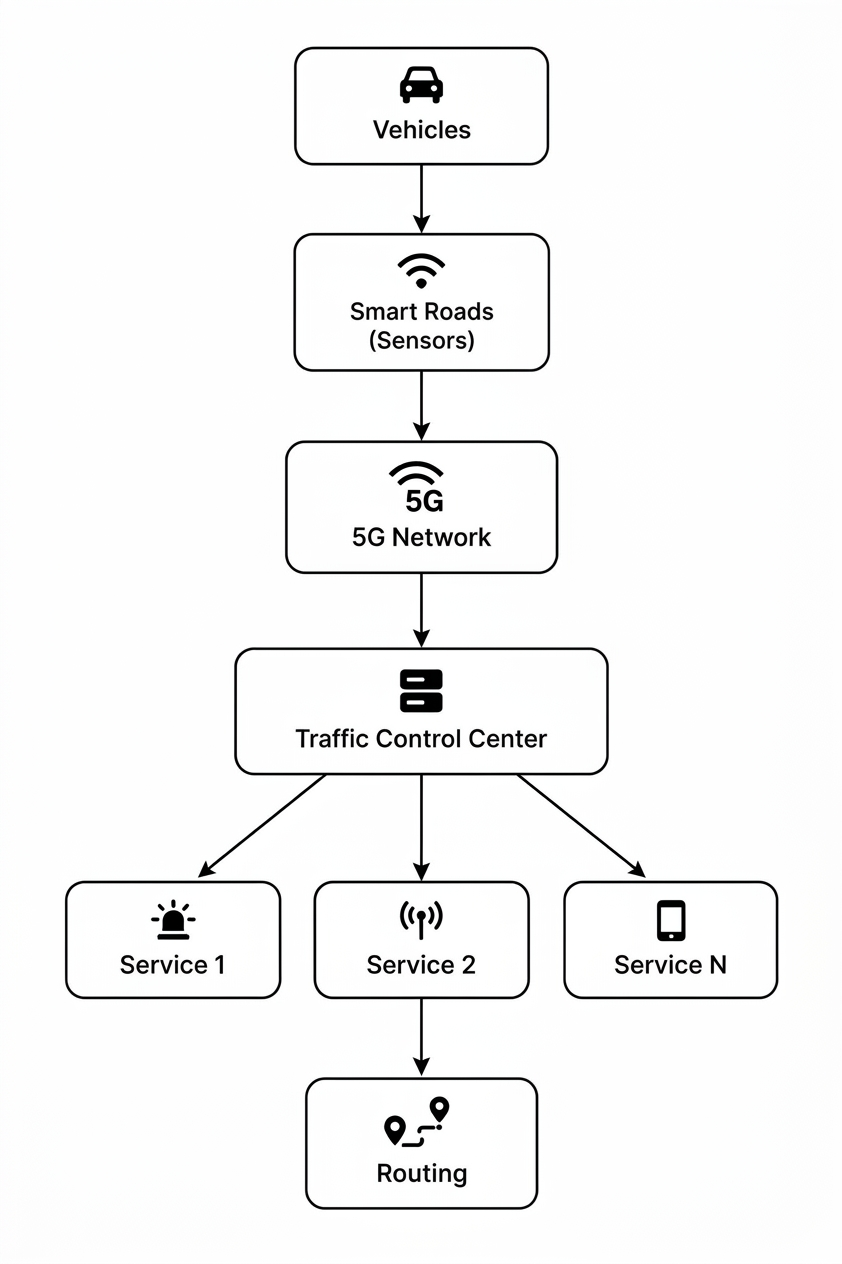
\includegraphics[width=0.72\linewidth]{image-009.png}
\caption{Smart Manufacturing and Industry 4.0}
\label{fig:manufacturing}
\end{figure}

Deploying 5G at scale requires substantial infrastructure investment, including small cells, fiber-optic backhaul, and edge computing facilities, as summarized in Table~\ref{tab:5g}. Spectrum allocation and management are similarly critical to successful 5G deployment, which relies on a combination of licensed, shared, and unlicensed spectrum bands \cite{r37}.

\begin{table}[!t]
\caption{5G Infrastructure Components}
\label{tab:5g}
\centering
\scriptsize
\setlength{\tabcolsep}{3pt}
\renewcommand{\arraystretch}{1.15}
\begin{tabularx}{\linewidth}{@{}>{\raggedright\arraybackslash}p{0.18\linewidth}XXXX@{}}
\toprule
\textbf{Components} & \textbf{Description} & \textbf{Role in Smart Applications} & \textbf{Real-World Examples} \\
\midrule
IoT Sensors & Devices that capture environmental, traffic, and infrastructure data. & Enable real-time monitoring of traffic, pollution, and public utilities. & Air quality sensor networks in Barcelona. \\

Data Centers & Facilities for processing, storing, and managing large volumes of urban data. & Support data analytics, decision-making, and service delivery. & Smart city data hubs in Amsterdam. \\

Cloud Computing & Scalable computing resources delivered over the internet. & Enables large-scale data processing, storage, and smart city applications. & Cloud-based urban management platforms in Singapore. \\

Urban Platforms & Integrated platforms that consolidate data from multiple city departments. & Facilitate data sharing, visualization, and coordinated decision-making. & Barcelona Urban Platform; FIWARE-based smart city platforms. \\
\bottomrule
\end{tabularx}
\end{table}

Digital infrastructure is thus anchored by IoT sensors, data centers, cloud computing, and urban data platforms, all of which together allow cities to manage themselves efficiently. IoT sensors monitor real-time environmental and traffic conditions -- air-quality monitoring in Barcelona is a representative example \cite{r39} -- while data centers provide the storage and analysis capacity needed for large-scale urban data, as illustrated by Amsterdam's smart data hubs \cite{r40}. Cloud computing supplies the internet-based, scalable resources that projects such as Singapore's Smart Nation initiative rely on to aggregate data across the city \cite{r41}, and Virtual Singapore's urban data platform offers centralized, real-time visualization that supports inter-departmental coordination for the benefit of residents \cite{r42}. Together, these digital elements are what make contemporary cities smart and sustainable. Fig.~\ref{fig:strategies} presents key strategies for optimizing digital infrastructure.

\begin{figure}[ht]
\centering
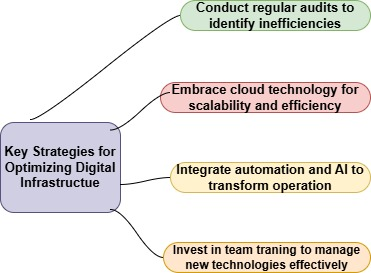
\includegraphics[width=\linewidth]{image-010.jpeg}
\caption{Key Strategies to Optimize Digital Infrastructure}
\label{fig:strategies}
\end{figure}

\subsection{Physical Infrastructure}
Adapting conventional infrastructure to the demands of smart cities requires integrating advanced technologies that improve efficiency, sustainability, and overall quality of life -- a transformation essential to addressing urban challenges and promoting sustainable growth. This subsection examines three critical areas of infrastructure adaptation: smart buildings, smart roads and highways, and modernized water and waste management systems.

\subsubsection{Smart Buildings}
Smart buildings use advanced technologies to optimize energy consumption, raise operational efficiency, and improve occupant comfort. Equipped with automated systems that control lighting, heating, ventilation, air conditioning (HVAC), and security, and built around the integration of IoT, data analytics, and energy management tools, smart buildings play a key role in advancing the sustainability objectives of smart cities. Their core components are Energy Management Systems (EMS), Building Management Systems (BMS), and sustainable design.

Energy Management Systems track and regulate energy usage in real time, optimizing consumption, minimizing waste, and reducing operational expenses; automated lighting that adjusts to occupancy and available natural light is a representative example of the resulting energy savings.

Building Management Systems integrate a building's various subsystems -- lighting, HVAC, and security -- into a single cohesive platform, enabling efficient management and real-time monitoring that improves both operational efficiency and occupant comfort.

Smart buildings also prioritize sustainability through energy-efficient design, renewable energy sources, and eco-friendly materials, incorporating features such as green roofs, rainwater harvesting, and energy-efficient windows.

The Edge in Amsterdam stands as one of the world's most advanced smart buildings, combining an efficient energy management system, automated lighting, and eco-friendly design; the broader development of smart urbanism in Amsterdam similarly emphasizes sustainable building practices that integrate smart technologies to enhance urban living while reducing environmental impact \cite{r46}. One World Trade Center in New York City incorporates a range of green technologies, including energy-efficient systems and advanced building management strategies aligned with LEED certification principles \cite{r47}.

Integrating smart technologies into buildings nonetheless requires significant up-front investment. Interoperability -- ensuring that different smart systems and devices work seamlessly together -- demands careful planning and standardization, and the collection and analysis of building-system data raises privacy and security concerns that call for robust data protection measures.

\subsubsection{Smart Roads and Highways}
Smart roads and highways use sensors, intelligent signaling systems, and real-time data analytics to improve traffic management, enhance highway safety, and reduce road congestion.

Sensors and cameras installed along roads capture real-time information on traffic, speed, and road conditions, which is used to track traffic patterns, identify congestion, and dynamically regulate traffic signals, as shown in Fig.~\ref{fig:roads}.

\begin{figure}[ht]
\centering
\begin{tabular}{@{}c@{}}
{\textbf{Vehicles}} (Cars / Trucks / Buses)\\
$\updownarrow$ (V2V Communication)\\
\textbf{Smart Road Infrastructure}\\
(Sensors, Cameras, Smart Signals, Toll)\\
$\downarrow$\\
\textbf{5G Network}\\
$\downarrow$\\
{\textbf{Traffic Control Center}}\\
(AI + Data Analytics)\\
$\downarrow$\\
Emergency / Smart Signals / User Apps\\
(Navigation Services)\\
$\downarrow$\\
{\textbf{Route Optimization System}}
\end{tabular}
\caption{Smart Roads and Highways}
\label{fig:roads}
\end{figure}

Traffic management systems that combine real-time information with adaptive control can reduce congestion in urban road networks \cite{r48}. Smart traffic lights use sensor data to adjust signal timing to current conditions, reducing waiting times and emissions from idling vehicles; research on adaptive traffic signal control confirms that such strategies can reduce both travel times and fuel consumption in congested urban networks \cite{r49}.

Vehicle-to-Infrastructure (V2I) communication allows vehicles to exchange information with roadside sensors and traffic lights, as depicted in Fig.~\ref{fig:v2i}.

\begin{figure}[ht]
\centering
\begin{tabular}{@{}c@{}}
{\textbf{Vehicle}} (Onboard Unit - OBU)\\
$\downarrow$\\
\textbf{Roadside Unit (RSU)}\\
(Traffic Signals / Sensors / Cameras)\\
$\downarrow$\\
\textbf{5G Network}\\
$\downarrow$\\
{\textbf{Control Center}} (Traffic Management)\\
$\downarrow$\\
{\textbf{Smart Signals}}\\
$\downarrow$\\
{\textbf{Driver Alerts}}\\
(Navigation / Warnings / Updates)
\end{tabular}
\caption{Vehicle-to-Infrastructure (V2I) Communication}
\label{fig:v2i}
\end{figure}

This technology supports applications such as traffic signal priority, collision avoidance, and real-time route adjustment; V2I communication enhances both safety and efficiency and has the potential to reduce the number of traffic accidents \cite{r50}. The Los Angeles Smart Corridor exemplifies an integrated traffic management system that combines real-time signal control and dynamic message displays to coordinate freeway and arterial traffic, reducing congestion and travel delays \cite{r51}, while the Barcelona Smart Traffic Management System combines traffic sensors, intelligent signaling, and data analysis to improve traffic flow and reduce congestion in that city \cite{r52}.

Smart roads and highways nonetheless face real limitations: implementation requires high up-front expenditure on infrastructure and technology; the large-scale collection and management of traffic data raises privacy and data-security concerns; and integrating new technologies with existing traffic management systems remains a complex undertaking.

\subsubsection{Water and Waste Management Systems}
Smart water and waste management systems combine sensors, data analytics, and automation to maximize the efficiency of water delivery and waste collection while minimizing pollution and environmental impact, as shown in Fig.~\ref{fig:water}.

\begin{figure}[ht]
\centering
\begin{tabular}{@{}c@{}}
\textbf{Water Source / Waste Generation}\\
(River / Household / Industry)\\
$\downarrow$\\
{\textbf{Sensors \& IoT Devices}}\\
(Level, Quality, Flow)\\
$\downarrow$\\
\textbf{5G Network}\\
$\downarrow$\\
{\textbf{Control Center}} (Monitoring \& AI)\\
$\downarrow$\\
{\textbf{Water System}} (Treatment) \quad {\textbf{Waste System}} (Collection)\\
$\downarrow$ \hfill $\downarrow$\\
\textbf{Clean Water Supply} \hfill \textbf{Recycling / Disposal}\\
$\downarrow$ \hfill $\downarrow$\\
\textbf{Consumers} \hfill \textbf{Environment}
\end{tabular}
\caption{Smart Water and Waste Management Systems}
\label{fig:water}
\end{figure}

Smart water meters provide real-time data on water usage, enabling accurate and timely billing, faster leak detection, and better management of water resources; research on smart water metering confirms that such meters can reduce non-revenue water and improve operational efficiency \cite{r53}. Smart waste management systems use bin-level sensors to monitor fill levels and optimize collection routes, reducing the frequency of collections, operational costs, and emissions from collection trucks, as research on IoT-enabled smart waste management has shown \cite{r54}. In water treatment plants, membrane filtration, ultraviolet disinfection, and real-time monitoring together improve water quality and ensure compliance with safety standards; studies of advanced water treatment technologies confirm that these processes improve water quality while reducing treatment costs \cite{r55}.

Singapore has implemented a smart water grid that uses sensors and data analytics to manage and monitor water supply, improving efficiency and reducing leakage \cite{r56}, while Rome has installed a smart waste management system that uses sensors to monitor waste levels and optimize collection timing, reducing costs and improving efficiency \cite{r57}.

Implementing smart water and waste management systems nonetheless requires significant infrastructure investment, and the collection and analysis of data from these systems raises data privacy and security concerns that must be addressed as existing systems are upgraded.

\subsection{Urban Planning and Design}
Integrating smart technologies into city planning is key to creating urban environments that are efficient, sustainable, and livable. Modern technologies allow cities to optimize their physical settings, raise quality of life, and resolve contemporary urban dilemmas, an approach that in practice means embedding intelligent technologies into mixed-use development, green space design, and sustainable urban planning.

\subsubsection{Mixed-Use Developments}
Mixed-use developments that incorporate smart technologies integrate residential, office, commercial, and recreational facilities within a single location, improving accessibility, reducing travel time, and promoting sustainable urban living, and thereby enhancing the convenience, efficiency, and overall well-being that smart cities aim to deliver.

Such developments rely on built-in infrastructure systems, including smart energy systems, intelligent transport systems, and centralized waste management, that make urban life more efficient and lower its environmental footprint; research on land use and transportation confirms that mixed-use development shortens commute times, reducing congestion and greenhouse gas emissions \cite{r58}. Smart buildings within mixed-use developments rely on automation systems to control energy use, lighting, and HVAC, improving comfort while lowering operating expenses and advancing sustainability goals; research on building energy use confirms that smart building systems can substantially improve energy efficiency and reduce operating costs \cite{r59}. Mixed-use developments also support smart mobility solutions -- electric vehicle charging stations, bike-sharing platforms, and built-in public transportation -- that are more environmentally friendly and reduce reliance on private vehicles; research on mixed-use development confirms that projects integrating mobility solutions such as public transport and bike-sharing reduce car dependence \cite{r60}.

Hudson Yards in New York implemented a large-scale mixed-use project that combines modern building management systems, energy-saving infrastructure, and smart mobility, transforming the neighborhood into a modern urban district with reduced commuting requirements \cite{r61}. Marina Bay Sands in Singapore similarly combines residential, commercial, and entertainment functions within a development built around energy-efficient infrastructure, intelligent transport solutions, and integrated infrastructure that together improve urban life and sustainability \cite{r62}. Table~\ref{tab:mixed} summarizes key findings on mixed-use development across countries.

\begin{table*}[!t]
\caption{Key Findings of Mixed-Use Developments in Various Countries}
\label{tab:mixed}
\centering
\scriptsize
\setlength{\tabcolsep}{3pt}
\renewcommand{\arraystretch}{1.15}
\begin{adjustbox}{width=\textwidth}
\begin{tabular}{@{}l
p{0.16\textwidth}
p{0.15\textwidth}
p{0.16\textwidth}
p{0.16\textwidth}
p{0.19\textwidth}
p{0.18\textwidth}@{}}
\toprule
\textbf{Ref} & \textbf{Study Area / Country} & \textbf{Type of Development} & \textbf{Key Components} & \textbf{Smart Technologies Used} & \textbf{Key Findings} & \textbf{Limitations} \\
\midrule
{[73]} & Global & Mixed-use urban developments & Residential, commercial, public spaces & Smart infrastructure, energy systems & Improves sustainability, economic activity & Lacks real-time implementation data \\
{[74]} & Europe & Mixed-use projects & Housing, offices, retail & Urban planning tools & Enhances social interaction, land efficiency & Policy complexity \\
{[75]} & Asia / Global & Urban megaprojects & Multi-functional urban zones & Smart planning frameworks & Large-scale mixed-use improves urban efficiency & High cost, long timelines \\
{[76]} & Global & Smart city development & Integrated urban systems & IoT, data analytics, cloud & Sustainability + smart governance & Data privacy concerns \\
{[77]} & Global & Smart sustainable cities & Infrastructure + services & IoT, AI, big data & Improves resource optimization & Implementation complexity \\
{[78]} & Global & Research trends & Urban systems & Digital technologies & Growing focus on sustainability \& mixed-use & Limited empirical validation \\
{[79]} & Europe & Smart construction & Real estate + infrastructure & Industry 4.0, IoT & Smart construction supports mixed-use growth & Technology adoption barriers \\
{[80]} & Middle East & Smart housing & Residential + community services & Smart home tech, energy systems & Enhances quality of life & Cost constraints \\
{[81]} & Global & Smart city frameworks & Urban planning systems & ICT, governance platforms & Mixed-use is core to smart urbanism & Conceptual focus \\
{[82]} & Global & Compact urbanism & Dense mixed land use & Data-driven planning & Supports sustainability \& mobility & Limited case-specific analysis \\
\bottomrule
\end{tabular}
\end{adjustbox}
\end{table*}

Mixed-use development is not without its limitations, including land-use conflicts, economic uncertainty, and the complexity of managing multiple functions within a single project. The up-front cost of smart technologies and mixed-use planning is substantial, and developers and municipalities must navigate complex zoning rules and approval processes that can slow project timelines.

\subsubsection{Green Spaces and Sustainable Urban Design}
Green spaces are a critical component of sustainable urban design, improving livability and environmental quality by reducing pollution, regulating temperature, and supporting biodiversity in rapidly developing cities. Integrating green corridors, parks, and urban forests supports both human well-being and ecological balance, contributing to healthier, smarter, and more resilient urban environments that use resources efficiently while preserving natural systems, improving air quality, mitigating urban heat islands, and offering residents recreational space. Research confirms that urban greening helps regulate urban temperatures and reduce stormwater runoff \cite{r63}. This design philosophy also emphasizes renewable resources, waste reduction, and green construction, incorporating principles such as rainwater collection, passive solar design, and renewable energy use.

\begin{table}[!t]
\caption{Revenue for Smart Cities 
\texttt{(Source: https://www.statista.com/})}
\label{tab:revenue}
\centering
\begin{tabular}{@{}cc@{}}
\toprule
\textbf{Year} & \textbf{Revenue in Billion USD (US\$)}\\
\midrule
2018 & 32.81\\
2019 & 38.99\\
2020 & 42.02\\
2021 & 49.22\\
2022 & 54.9\\
2023 & 67.18\\
2024 & 72.52\\
2025 & 79.94\\
2026 & 88.11\\
2027 & 96.75\\
2028 & 106.3\\
2029 & 115.3\\
\bottomrule
\end{tabular}
\end{table}

Buildings and the built environment account for a large share of global energy use and greenhouse gas emissions, and improved design can substantially reduce both \cite{r64}. Access to green space, meanwhile, has been shown to improve mental health, reduce stress, and promote physical activity, and is associated with reduced symptoms of anxiety and depression \cite{r65}.

The High Line, an elevated linear park built through a former industrial corridor in New York City, illustrates how green infrastructure can improve urban appearance, provide recreational space, and stimulate local economic growth \cite{r66}. The Vauban district in Freiburg, Germany, integrates car-free transit, green space, and low-energy buildings into a coherent sustainable urban district \cite{r67}. The long-term success of such projects depends on developing green spaces and environmentally friendly buildings capable of withstanding both regional climate conditions and the broader pressures of global warming. Tables~\ref{tab:mixed} and~\ref{tab:revenue} together illustrate the environmental and economic impact of these initiatives.

\section{Innovation and Technology in Smart Cities}
Rapid population growth continues to drive demand for better infrastructure, resource management, and sustainability, and cutting-edge technologies -- artificial intelligence, the Internet of Things, big data analytics, and cloud computing -- are central to making cities more efficient, responsive, and sustainable in response. These technologies support the collection and interpretation of real-time information and the decision-making that follows, improving sectors as varied as healthcare, transportation, energy, and public safety. This section examines how innovation and technology are set to reshape the future of urban life.

The scale at which these technologies can gather, analyze, and act on data improves decision-making, trend forecasting, and overall urban functionality across public safety, transportation, and city management. Innovation in smart cities means rethinking conventional infrastructure and amenities as much as adopting new technology outright: efficient smart-grid energy distribution, waste management systems that support higher recycling rates, and intelligent transportation systems that ease congestion are all part of this broader shift. The integration of online services for citizen engagement further allows residents to participate with municipal organizations in real time, offering input and taking part in decision-making; beyond fostering a stronger sense of community, this participatory approach helps ensure that the needs and preferences of local populations are reflected in smart city development. Technological innovation also drives economic development in smart cities by attracting capital, creating jobs, and enabling new industries, even as the broader focus on efficiency, sustainability, and resilience must contend with global challenges of social inequality, climate change, and resource depletion.

\subsection{Information and Communication Technology}
ICT lies at the core of smart city operations, enabling data to be collected, processed, and delivered efficiently to improve city management and decision-making. Barcelona has been a pioneer in integrating ICT into its smart city programs, deploying a comprehensive urban platform that combines data sources ranging from social media to sensor networks to monitor and provide urban services such as waste collection, traffic management, and energy consumption tracking. This integration has produced significant reductions in energy and water use and helped position Barcelona at the forefront of smart city innovation internationally \cite{r68}.

\subsection{Smart City Systems}
The Internet of Things comprises a web of devices and sensors that collect and transmit data on urban conditions such as traffic patterns, air quality, and energy usage. IoT plays a significant role in managing city infrastructure and enabling real-time inspection, allowing authorities to respond quickly to emerging issues and use resources more efficiently.

IoT-based dimming systems illustrate this potential by transforming conventional lighting into a smart, adaptive, and energy-efficient system. By integrating sensors, controllers, and cloud intelligence, such lighting responds to real-world conditions, substantially reducing energy consumption while improving user comfort. Fig.~\ref{fig:iot-dimming} shows a representative IoT-based smart lighting architecture.

\begin{figure}[ht]
\centering
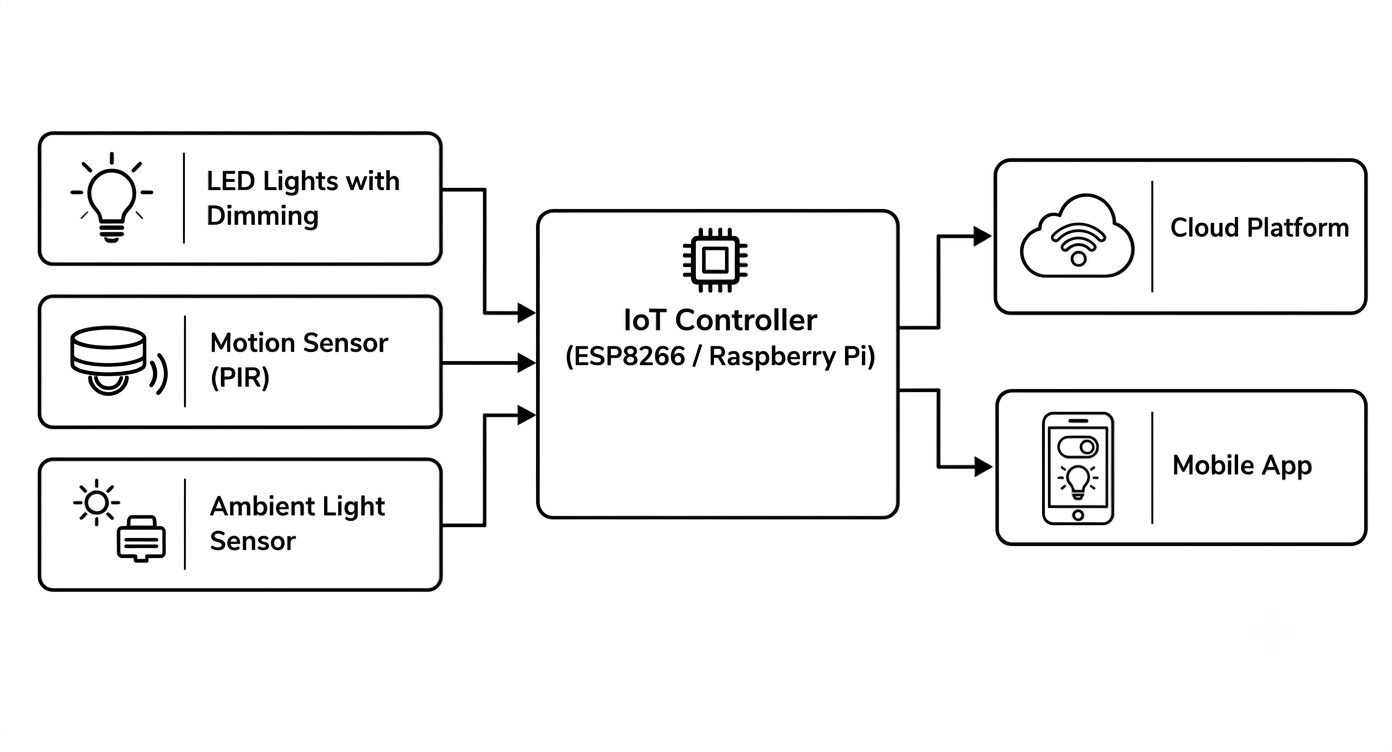
\includegraphics[width=\linewidth]{image-011.png}
\caption{IoT-based Smart Lighting (Dimming) System}
\label{fig:iot-dimming}
\end{figure}

Singapore's Smart Nation initiative demonstrates the concept of a smart city in practice, using IoT to monitor and control urban infrastructure efficiently. Among its notable projects is a national sensor network that tracks traffic conditions and waste bin levels across the city, supporting both urban planning and service delivery; AI-based traffic management has similarly been proposed and piloted to reduce congestion on Singapore's road network \cite{r69}.

Big Data Analytics has emerged as a key technology enabling cities to derive meaningful insight from the large volumes of data generated across sectors, processing and analyzing this data to identify trends, patterns, and other perspectives that enhance urban services and inform decision-making. Applications range from emergency response and energy distribution to traffic forecasting, and officials increasingly base predictions and decisions on data drawn from social media, sensors, and municipal databases.

Cities worldwide are increasingly turning to Big Data Analytics to improve infrastructure, healthcare, and urban planning. New York City has used big data analytics to improve the effectiveness of city departments and strengthen public safety: its Domain Awareness System draws on social media, police databases, and CCTV cameras to support real-time surveillance and crime response \cite{r18}, while big data analytics has also been applied to optimize the city's waste management system and improve recycling rates \cite{r70}.

Building on IoT and Big Data Analytics, Artificial Intelligence transforms this massive volume of data into practical, actionable information. AI-driven systems support real-time monitoring, predictive analysis, and automation, improving the efficiency and sustainability of smart governance, smart mobility, smart environment, smart healthcare, smart economy, and smart living. Case studies from around the world illustrate AI's application in these domains, drawing on techniques such as machine learning, deep learning, and computer vision that have become embedded across smart city systems -- evidence that AI functions less as a single-purpose tool than as a pervasive, integrative technology linking every element of a smart city, even as it raises real concerns about data privacy, infrastructure cost, and standardization \cite{r6}.

Hangzhou, China -- the home city of Alibaba -- has implemented an AI-powered "City Brain" project to oversee its urban infrastructure, analyzing data from more than 1,000 cameras and sensors across the city. The result has been optimized traffic flow, reduced congestion, faster emergency response, and improved public safety \cite{r71}.

Blockchain technology offers a secure, decentralized platform for managing data transparently and without intermediaries, and has become an important part of smart city infrastructure by enhancing data security, trust, and coordination among stakeholders -- governments, developers, and citizens alike \cite{r92,r93}. Blockchain is also compatible with the Internet of Things, ensuring secure communication and rapid data exchange across city-level infrastructure \cite{r94}. In mixed-use developments, blockchain can improve operational efficiency through smart contracts, secure property transactions, and energy management systems \cite{r95,r97}, although high implementation costs, scaling challenges, and regulatory uncertainty continue to limit its adoption in large-scale smart city projects \cite{r97,r96}.

Dubai has announced a strategy to become a fully blockchain-based government and has already deployed the technology across sectors including healthcare, transportation, and real estate. The Dubai Land Department, for instance, uses blockchain to expedite real estate transactions, cutting the time needed to close a deal from weeks to a few hours, while blockchain has also improved the transparency and security of the city's digital identity management system \cite{r72}.

\begin{figure*}[!t]
\centering
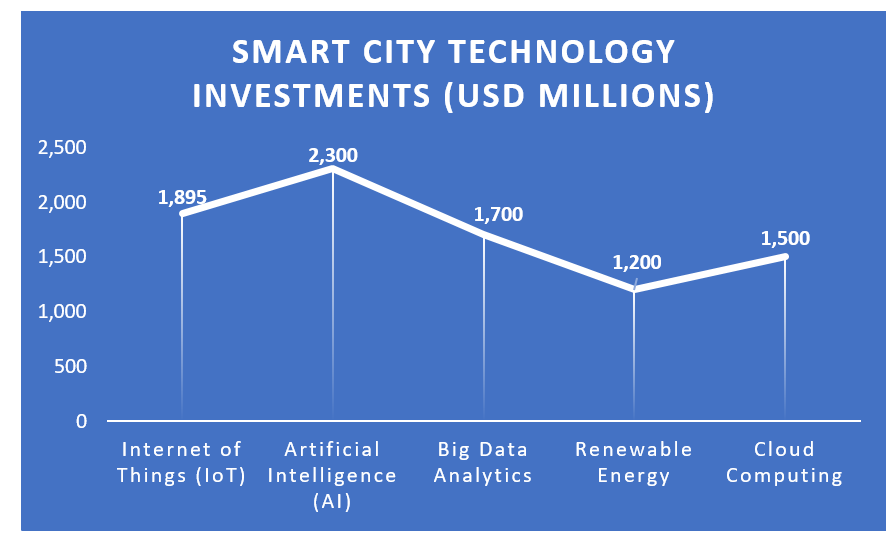
\includegraphics[width=0.8\textwidth]{image-012.png}
\caption{Smart City Investments}
\label{fig:investments}
\end{figure*}

\begin{figure*}[!t]
\centering
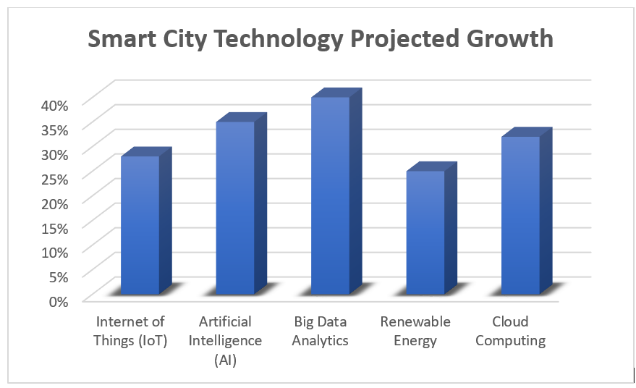
\includegraphics[width=0.8\textwidth]{image-013.png}
\caption{Smart City Projected Growth}
\label{fig:growth}
\end{figure*}

Smart governance refers to the use of technology to improve government operations, and reflects how inclusive, effective, transparent, and participatory a smart city's decision-making processes are. Digital platforms and resources allow governments to broaden citizen participation, streamline administrative processes, and deliver services more effectively, encompassing activities such as digitizing public services, using data analytics to inform policy decisions, and integrating citizen feedback into governance.

Authorities routinely draw on real-time data from multiple sources to manage resources, evaluate municipal infrastructure, and address emerging problems, while smart governance further promotes transparency by making government data publicly available and allowing citizens to track program progress -- an openness that builds trust between citizens and government by creating a genuinely participatory governance process.

Seoul, South Korea, has integrated technology across every facet of its city management through a smart governance system that offers more than 1,000 datasets on its Open Data Plaza, allowing citizens to track government activity and engage in policy discussion. Seoul residents can also vote directly on municipal issues through the mVoting smartphone application; together, these initiatives have driven public participation in governance activities above 50 percent \cite{r99,r34}.

E-government services are digital platforms that give citizens access to public services while lowering bureaucracy, improving accessibility, and speeding service delivery. By digitizing government functions, smart cities give citizens an easier, more efficient way to engage with government entities, whether through online tax filing, permit applications, or requests for social services. This transition saves time for both citizens and government workers by eliminating the need for in-person office visits, while also ensuring that residents in rural or underserved areas -- and citizens generally, given round-the-clock access -- can obtain the services they need with greater freedom and convenience \cite{r73,r100}.

Estonia, widely regarded as the most technologically advanced e-government in the world, exemplifies this model. Through the e-Estonia project, residents can access services such as voting and tax filing entirely online, and nearly all public services can be completed digitally, saving the government money while giving residents faster, more effective access to public services \cite{r74,r101}.

Citizen participation platforms represent another category of digital technology that enables residents to collaborate with local governments, raise concerns, and take part in decision-making. By giving citizens a voice in how their city is managed, these platforms -- which may include social media, smartphone applications, and online discussion forums -- help ensure that city planning reflects the community's actual needs and preferences, and that citizen demands are identified and addressed through two-way communication between the public and government.

Better Reykjavik is a leading example of an effective citizen participation platform. Launched in 2010, the online platform allows residents to propose, debate, and vote on ideas to improve the city, with the most popular proposals reviewed and, where feasible, implemented by the city council. By 2023, more than three-quarters of Reykjavik's residents had registered on the platform, and more than 800 citizen-proposed initiatives had been successfully implemented, strengthening transparency and trust in local government \cite{r75,r102}.

Smart mobility systems apply advanced technologies and novel solutions to transportation networks in smart cities, aiming to create a smooth, efficient, and sustainable transport system that reduces congestion, minimizes environmental impact, and improves the passenger experience through autonomous vehicles, intelligent public transportation, and shared mobility solutions. As a core component of smart cities, smart mobility plays a substantial role in driving economic growth, reducing pollution, and improving quality of life.

Autonomous vehicles (AVs) in smart cities are self-driving vehicles equipped with advanced sensors, AI software, and communication systems that allow them to move and operate independently, aiming to reduce traffic congestion and accidents while improving the use of road capacity. AVs exchange information with other vehicles, intelligent traffic lights, and city systems to make real-time decisions that prevent congestion, select efficient routes, and regulate traffic flow across the network, largely eliminating the human error responsible for most accidents while maintaining safe distances and responding quickly to unforeseen obstacles; they can also be integrated into public transport and shared mobility services to improve urban transportation efficiency further.

Phoenix, Arizona, has become a leader in autonomous vehicle testing in the United States: Waymo, a subsidiary of Alphabet Inc., has operated a fleet of self-driving cars in the city since 2017, using advanced lidar, radar, and camera systems to navigate autonomously. The deployment has shown promising results in reducing traffic congestion and accidents, and studies of Waymo's operations report that its autonomous vehicles have driven tens of millions of miles on public roads with lower crash rates than human-driven vehicles \cite{r76,r103}.

Smart public transit systems use real-time data, IoT sensors, and advanced algorithms to optimize public transportation networks, giving commuters real-time tracking of buses, trains, and other transit modes along with accurate arrival times, route information, and service updates through mobile apps and digital displays. These live updates shorten waiting times, improve route coverage, and enhance the reliability of public transportation, while data analytics allows transit agencies to forecast demand, optimize schedules, and reduce operating costs; by analyzing passenger flows, cities can adjust routes and schedules to better match demand, using resources more efficiently and reducing delays for passengers.

London's Transport for London (TfL) has implemented a modern smart transit network that draws on real-time information to manage its extensive bus, train, and tram network. The city's Countdown system makes real-time bus arrival information available at stops and online, helping passengers plan their journeys more effectively, while TfL uses data analytics to manage bus schedules and improve service reliability and quality. Smart ticketing systems, including the Oyster card and contactless payment, have further streamlined public transportation across London \cite{r77,r104}.

Shared mobility services -- car-sharing, bike-sharing, and ride-hailing -- offer flexible transportation options to urban residents, easing congestion by reducing the number of privately owned vehicles on the road and promoting sustainability through shared resource use; these services are typically integrated with public transit to create an efficient multimodal transportation system \cite{r11}. Car-sharing platforms such as Zipcar and Turo allow commuters to rent vehicles for short trips, reducing the number of privately owned cars on the road, while bike-sharing programs such as Citi Bike in New York and Mobike in China give users convenient access to bicycles and more eco-friendly travel options. Ride-hailing services such as Uber and Lyft offer on-demand rides that are often more convenient and affordable than traditional taxis.

Copenhagen has emerged as a pioneer in shared mobility, placing strong emphasis on sustainable transportation. The city's bike-sharing app, Bycyklen, provides GPS-enabled electric bicycles with smart locks that make bikes easy to find and rent, an initiative that has been widely adopted and now records millions of rides each year. Copenhagen has also integrated car-sharing services with its public transit system, offering flexible travel options to residents and visitors alike; this strong emphasis on shared mobility has helped reduce CO$_2$ emissions and road traffic congestion in the city, supporting its goal of achieving carbon neutrality by 2025 \cite{r78,r105}.

Smart energy systems play a vital role in developing sustainable smart cities by enabling the efficient, intelligent use of energy resources, reducing environmental impact, enhancing reliability, and supporting economic growth. These systems draw on advanced technologies to optimize energy distribution, integrate renewable energy sources, and implement energy storage solutions that balance supply and demand, helping cities reduce their carbon footprint, improve energy efficiency, and provide a consistent energy supply to public and commercial sectors alike.

Smart grid systems are modern energy distribution networks that use digital communication technologies to monitor and manage electricity flow between producers and consumers in real time. Unlike conventional power grids, which rely on one-way communication, smart grids support two-way interaction, enabling more efficient energy distribution, improved load balancing, and faster response to power outages through advanced sensors, smart meters, and automated control systems that supply live data on energy usage and distribution. This information is used to optimize electricity delivery, minimize transmission losses, and better manage demand, while smart grids also support the integration of renewable energy sources by dynamically adjusting electricity flow to align supply with demand, reducing reliance on fossil-fuel-based backup power. Amsterdam is a leading adopter of smart grid technology: through the "Amsterdam Smart City" pilot project, the city connects households, businesses, and renewable energy sources such as rooftop solar panels, enabling real-time monitoring of household energy consumption and allowing households to adjust usage based on pricing signals and availability. The pilot has demonstrated reductions in energy consumption and a clear path toward greater use of renewable energy across the city \cite{r79,r106}.

Integrating renewable energy -- solar, wind, and hydroelectric power -- into the energy systems of smart cities is critical to minimizing greenhouse gas emissions and ensuring long-term sustainability, though the variability of renewable output, driven by weather conditions, complicates its integration into smart grids. Cities address this challenge through sophisticated forecasting techniques, energy management systems, and flexible grid infrastructure that ensure renewable energy is incorporated efficiently, with smart grids playing an important role in dynamically directing energy to where it is needed and storing surplus for future use. Freiburg, Germany -- known as the "Solar City" -- exemplifies successful renewable energy integration, generating a substantial share of its electricity from rooftop solar panels on government buildings and designing its energy system to adapt dynamically to solar availability. Freiburg's sustained commitment to renewable energy has made it one of the most sustainable cities in Europe \cite{r80,r107}.

Energy storage systems help balance energy supply and demand in smart cities, particularly where renewable energy sources are being integrated, by accumulating excess power during periods of low demand or high renewable output and releasing it when demand exceeds supply. These systems reduce dependence on fossil fuels, stabilize the grid, and provide a consistent power source by minimizing variation in energy production, drawing on technologies that include thermal energy storage, pumped hydro, and battery storage, and are often paired with renewable energy systems and smart grids to create a more adaptable, sustainable energy platform.

The Tesla Powerpack installation at Hornsdale, South Australia, ranks among the largest battery energy storage systems in the world, built to address energy supply challenges and support more effective integration of renewable energy into the South Australian grid. By storing surplus wind farm energy and releasing it during peak hours, the system helps avoid blackouts and grid imbalances caused by fluctuating renewable supply, and has demonstrated the feasibility of large-scale energy storage as an enabler of renewable energy integration \cite{r81,r108}.

\section{Connecting Smart Cities Worldwide}
Connecting smart cities worldwide is a global priority: as cities increasingly embed systems for data, connectivity, and automation into their infrastructure and services, establishing universal standards and cross-border cooperation becomes essential to linking these urban centers together in pursuit of greater efficiency, sustainability, and resident well-being.

International partnerships and alliances have formed to promote innovation, guarantee compatibility, and share proven strategies, and examples from Singapore to New York illustrate how these connected urban ecosystems use technology to solve pressing challenges, improve daily life, and stimulate economic growth. This section explores how smart cities are interconnected at a global level -- an interconnectedness that enables seamless collaboration, knowledge sharing, and coordinated development across regions -- focusing on the standards, collaborative efforts, and initiatives that make this integration possible.

\subsection{Global Standards and Interoperability}
The interoperability of technologies deployed across smart cities worldwide depends on universal standards, which make cooperation between municipalities substantially more efficient. Fig.~\ref{fig:standards} illustrates the global standardization landscape.

\begin{figure*}[!t]
\centering
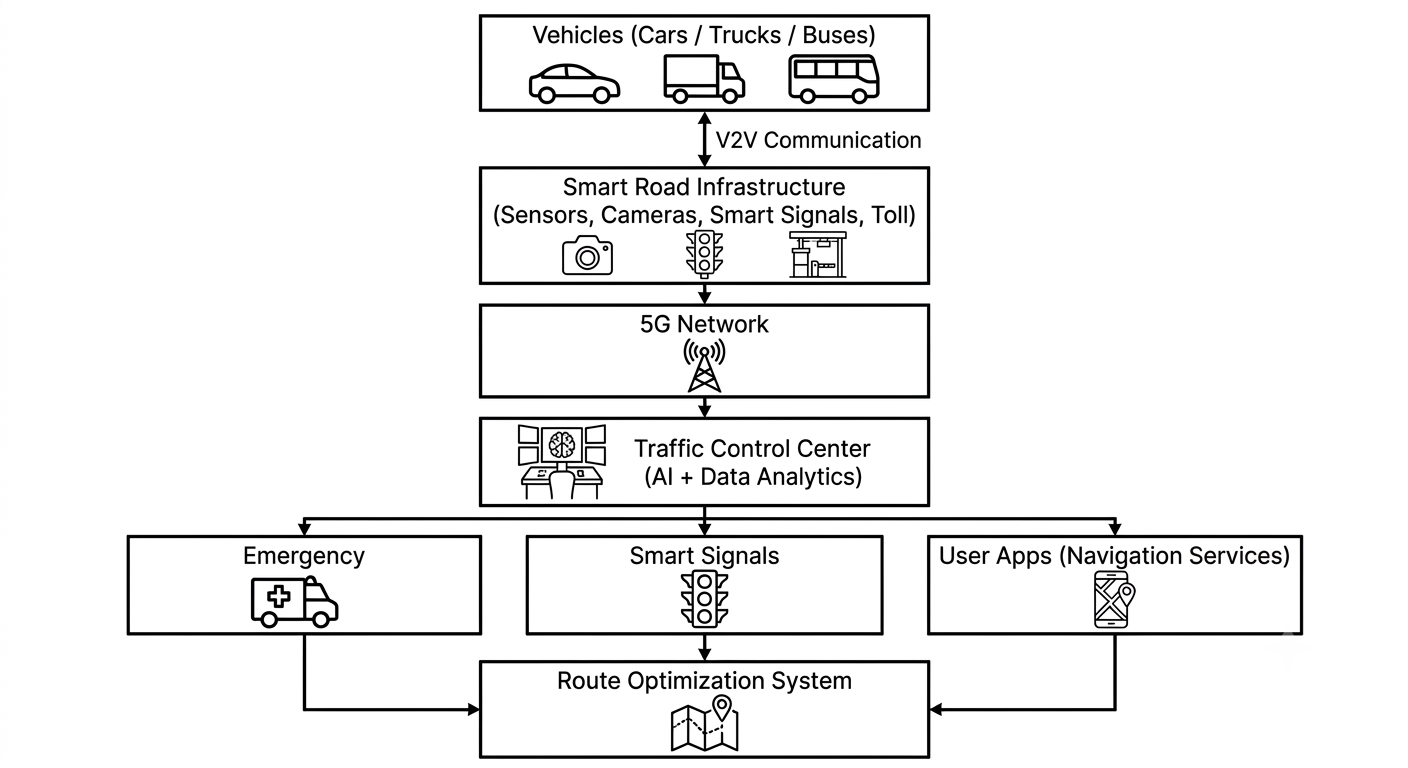
\includegraphics[width=0.8\textwidth]{image-014.png}
\caption{Global Standards and Interoperability}
\label{fig:standards}
\end{figure*}

Organizations such as the International Organization for Standardization (ISO) develop major standards in this space, including ISO 37120 on urban performance and ISO 37122 on smart city indicators, while IEEE and oneM2M frameworks define critical interoperability standards for IoT systems \cite{r82}. These standards allow disparate technologies -- from transit networks to public health platforms -- to work together, letting cities deploy new solutions with minimal overhaul; adopting common standards and benchmarking frameworks in this way facilitates collaboration and knowledge sharing between municipalities \cite{r83}.

\subsection{International Collaborations and Partnerships}
Smart cities depend on international collaboration to share best practices, pool resources, and disseminate effective solutions. The Global Smart City Partnership Program (GSCP), supported by organizations including the World Bank and UN-Habitat, facilitates the global sharing of innovative frameworks and enables knowledge exchange on topics such as digital governance and urban mobility \cite{r94}; such collaborative measures accelerate urban innovation while reducing operational costs through shared global resources \cite{r86}.

International initiatives such as the United for Smart Sustainable Cities (U4SSC) program, coordinated by the International Telecommunication Union, similarly aim to develop a unified approach for cities seeking to improve their technological environments, driving the creation of common indicators and standards for smart sustainable development \cite{r83,r85}. Such initiatives allow cities to align their growth with global sustainability and technological goals in ways that remain scalable over the long term.

City networks such as C40 Cities and the Global Covenant of Mayors enable municipalities to cooperate on urgent global issues, including climate action and sustainability. C40 Cities represents nearly 100 major cities pursuing climate action through coordinated city strategies, while the Global Covenant of Mayors unites more than 10,000 cities around climate and energy initiatives. These partnerships facilitate information sharing, joint planning, and common policy formulation, allowing cities to act more quickly on shared global challenges \cite{r86,r109}.

The success of Singapore, Barcelona, Dubai, and New York illustrates what this kind of collaboration can achieve. Singapore's Smart Nation initiative sets the pace for how smart urban technologies can be embedded at scale, deploying IoT, AI, and big data across transit, healthcare, and administration, with public and private IoT systems networked citywide to improve the efficiency of public services \cite{r87,r110}; the Virtual Singapore digital model further supports a real-time platform that integrates environmental, population, and infrastructure data to improve city management.

Barcelona is similarly characterized by innovative city planning and intelligent transportation systems, with a citywide sensor network monitoring air quality, energy usage, and traffic; projects such as electric bike-sharing and smart parking have reduced congestion and improved urban mobility \cite{r88,r111,r35}, positioning Barcelona as one of the most sustainable and livable cities in Europe.

Dubai represents another notable success story, with its smart city strategy centered on blockchain and AI to build a more efficient, transparent administration. Numerous government services have been digitized through blockchain, reducing paperwork and accelerating service delivery, while AI-driven improvements have lowered administrative costs and cemented Dubai's status as a pioneer in smart governance \cite{r89,r112}. New York City, as part of its own global smart city initiative, focuses on sustainability and resilience, using technology to address climate change, public health, and urban resilience; among its resilience projects are real-time crisis management systems that allow the city to respond to emergencies faster and more effectively \cite{r90,r113}.

\section{SDGs and Global Smart City Initiatives}
Smart city development is closely aligned with the United Nations Sustainable Development Goals (SDGs), particularly SDG 11, which focuses on sustainable and inclusive cities. These goals promote efficient resource use, reduced environmental impact, and improved urban quality of life through smart technologies, and countries around the world are integrating SDG targets directly into their urban planning and governance frameworks. India's Smart Cities Mission, for example, emphasizes sustainable infrastructure, digital governance, and citizen-centric services, while similar initiatives in Singapore and the European Union focus on green mobility, energy efficiency, and data-driven urban management.

\subsection{Role of SDGs in Smart Cities}
Rapid global urbanization creates unprecedented challenges and opportunities for sustainable development. Cities remain the primary engines of economic growth and innovation even as they face mounting pressures from climate change, resource consumption, social inequality, and environmental degradation. The United Nations' 2030 Agenda for Sustainable Development -- and specifically SDG 11, which calls to "make cities and human settlements inclusive, safe, resilient, and sustainable" -- recognizes the central role of urban sustainability in achieving global sustainable development \cite{r114}.

Understanding how research communities are contributing to SDG 11 and its associated goals requires a multidisciplinary lens, since cities differ widely in their socio-ecological characteristics and the intricate relationships among the environmental, social, and economic dimensions of sustainability demand correspondingly broad analytical approaches \cite{r114}. Recent scholarship suggests that urban sustainability research has moved from a siloed approach toward a more holistic framework that recognizes the interconnection among diverse urban challenges \cite{r115}.

The emergence of smart city approaches and technology-linked policy has, in turn, added complexity to urban sustainability research \cite{r116}: the combination of digital technologies and data-driven methods for urban development has opened innovative opportunities for sustainable development while simultaneously raising questions about equity and accessibility \cite{r117}, spawning multiple research streams that examine how smart city solutions can advance several SDGs at once.

As this discourse evolves, increasing attention is being paid to how smart city frameworks can accelerate progress toward the SDGs. SDG 11 in particular has catalyzed a research shift toward technologically enhanced, data-driven, human-centric urban development, with smart cities increasingly positioned as enablers of broader sustainability goals -- through innovations in governance, environmental monitoring, and participatory platforms -- rather than as tools that merely address traditional urban issues such as mobility, waste, and energy. These integrative approaches, which also embed climate adaptation and mitigation considerations \cite{r118,r119}, reinforce the role that smart city planning plays in advancing the SDG agenda by offering scalable, adaptive urban solutions that move beyond siloed strategies.

\subsection{Country-Level Smart City Initiatives}
Countries around the world are implementing smart city initiatives aligned with sustainability and digital transformation goals \cite{r1,r120}. In India, the Smart Cities Mission focuses on improving urban infrastructure, governance, and quality of life through data-driven solutions \cite{r2,r121}, integrating technologies such as IoT and AI through Integrated Command and Control Centres that support real-time urban management \cite{r3,r122}. In Singapore, the Smart Nation initiative emphasizes digital governance, citizen engagement, and innovation-driven urban services \cite{r4,r123}.

The European Union promotes sustainable smart cities through the Horizon Europe program, targeting climate-neutral cities by 2030 \cite{r1,r120}, while global initiatives such as the G20 Smart Cities Alliance focus on developing standards for data governance and ethical technology use in cities \cite{r94}. Countries across Southeast Asia and Africa are similarly adopting smart city frameworks, supported by international organizations, to improve urban resilience and inclusivity \cite{r4,r123}. Together, these initiatives demonstrate the importance of integrating policy, technology, and sustainability in urban development \cite{r1,r120,r4,r123}, even though implementation varies considerably across countries owing to differences in economic capacity, governance structures, and infrastructure readiness \cite{r4,r123}. Overall, global smart city initiatives reflect a strong commitment to sustainable urban development aligned with the SDGs \cite{r1,r114,r120}.

\begin{table*}[!t]
\caption{Country-Level Smart City Initiatives}
\label{tab:country}
\centering
\scriptsize
\setlength{\tabcolsep}{4pt}
\renewcommand{\arraystretch}{1.15}
\begin{tabularx}{\textwidth}{@{}
>{\raggedright\arraybackslash}p{0.10\textwidth}
X
>{\raggedright\arraybackslash}p{0.16\textwidth}
>{\raggedright\arraybackslash}p{0.18\textwidth}
>{\centering\arraybackslash}p{0.10\textwidth}
>{\centering\arraybackslash}p{0.06\textwidth}
@{}}
\toprule
\textbf{Country} &
\textbf{Initiative} &
\textbf{Focus Area} &
\textbf{Key Technologies} &
\textbf{SDG Link} &
\textbf{Ref} \\
\midrule
India &
Smart Cities Mission &
Urban infrastructure modernization, digital governance, and citizen-centric services &
IoT, AI, GIS, smart mobility, and integrated command centers &
SDG 11 &
[120] \\

Singapore &
Smart Nation Initiative &
Digital governance, urban mobility, healthcare, and public services &
AI, Big Data, IoT, cloud computing, and digital identity platforms &
SDG 9, 11 &
[121] \\

European Union &
Horizon Europe – Climate-Neutral and Smart Cities Mission &
Climate neutrality, sustainable urban development, and energy transition &
Smart grids, digital twins, renewable energy systems, and IoT &
SDG 11, 13 &
[122] \\

Global &
G20 Global Smart Cities Alliance &
Policy harmonization, urban governance, and international collaboration &
Data standards, digital governance frameworks, and interoperability platforms &
SDG 16 &
[123] \\
\bottomrule
\end{tabularx}
\end{table*}

\subsection{Case Studies (India, Singapore, EU, UAE, USA)}
In India, the Smart Cities Mission demonstrates large-scale urban transformation through area-based development and IoT-enabled governance, as evidenced in cities such as Vadodara and Pune \cite{r122}. Singapore's Smart Nation initiative represents a leading global model, integrating AI, IoT, and national digital platforms to enhance urban services and citizen engagement \cite{r123}.

In the European Union, the Horizon Europe mission promotes climate-neutral cities by 2030 through smart energy systems, mobility solutions, and sustainable infrastructure \cite{r85}. The United Arab Emirates, particularly Dubai and Abu Dhabi, focuses on AI-driven governance, smart mobility, and blockchain-enabled public services as part of its digital transformation strategy \cite{r112}.

In the United States, cities such as New York emphasize resilience planning, smart infrastructure, and data-driven environmental monitoring to address climate risks \cite{r90,r113}. Across these regions, IoT, artificial intelligence, and big data analytics are widely adopted to improve urban efficiency and sustainability \cite{r4}, and case studies show that digital platforms and integrated infrastructure are key enablers of real-time decision-making and service delivery \cite{r106}. Implementation strategies nonetheless vary depending on governance models, economic capacity, and technological maturity \cite{r116}: developed regions tend to prioritize sustainability and climate neutrality, whereas developing countries emphasize infrastructure and service accessibility \cite{r101}. Overall, these global case studies show that successful smart city development requires integrating technology, policy frameworks, and sustainability goals \cite{r84}.

\section{Challenges and Future Directions}
As smart cities continue to evolve, addressing critical challenges becomes essential to achieving resilient, inclusive, and sustainable urban environments. Key challenges include privacy and security concerns, the need for inclusive and equitable access, the development of effective regulatory and policy frameworks, and the pursuit of long-term environmental and economic sustainability.

Smart cities offer substantial benefits in efficiency, sustainability, and living standards, but the pace of technological change brings with it problems that must be resolved for these gains to be sustained. Cybersecurity threats and the risk of personal data loss grow more serious as cities become increasingly interdependent, and the challenge of inclusiveness and equity cannot be overlooked, since the digital divide can leave certain groups unable to fully benefit from smart city innovations (Table~\ref{tab:challenges}).

\begin{table}[!t]
\caption{Challenges in Smart City Development}
\label{tab:challenges}
\centering
\scriptsize
\setlength{\tabcolsep}{3pt}
\renewcommand{\arraystretch}{1.15}
\begin{tabularx}{\linewidth}{@{}>{\raggedright\arraybackslash}p{0.20\linewidth}XXX@{}}
\toprule
\textbf{Challenge Area} & \textbf{Description} & \textbf{Key Solutions/Strategies} & \textbf{Notable Case Example} \\
\midrule
Data Privacy &
Concerns regarding the collection, sharing, and storage of citizens' personal data. &
Privacy-preserving mechanisms, data anonymization, strong encryption, and cybersecurity frameworks. &
GDPR implementation across European smart cities. \\

Financial Constraints &
High capital investment and long-term operational costs associated with smart city infrastructure. &
Public--private partnerships (PPPs), government funding, and international development grants. &
World Bank Smart City Partnership initiatives. \\

Regulatory Issues &
Rapid technological advancement often outpaces existing legal and regulatory frameworks. &
Adaptive policies, regulatory sandboxes, and technology-specific governance frameworks. &
Autonomous vehicle regulations in Arizona, USA. \\

Inclusivity and Equity &
Unequal access to digital infrastructure and smart city services among different population groups. &
Affordable digital access, digital literacy programs, and inclusive urban planning. &
"Digital Equity for All" initiative, New York City. \\
\bottomrule
\end{tabularx}
\end{table}

Effective regulatory and policy frameworks are necessary to govern new technologies without undermining public trust, and sustainability remains a major concern as cities work to balance technological gains against environmental protection. The future effectiveness of smart cities in becoming resilient, inclusive, and sustainable will depend on how well these problems are resolved.

Data privacy and cybersecurity have become central concerns as smart cities amass large volumes of information through IoT devices, sensors, and smart infrastructure. Cities rely on personal information to optimize services such as public transport, waste collection, and emergency response, which leaves these systems vulnerable to cyberattack; research on smart city security confirms that cities deploying extensive IoT, sensor, and smart infrastructure systems are increasingly exposed to cyberattacks and data breaches \cite{r91}. Guaranteeing data privacy is a related challenge, particularly under regulatory regimes such as the General Data Protection Regulation (GDPR) in the European Union and the California Consumer Privacy Act (CCPA) in the United States; cities should deploy strong encryption and anonymization strategies alongside data management systems that protect citizens' privacy rights \cite{r92}.

Inclusivity and equity are similarly major concerns in smart city technology development: the benefits of a smart city -- improved mobility, health, and service delivery -- should be accessible to every citizen regardless of socioeconomic status, yet access to smart city services in developing countries remains uneven owing to digital divides and infrastructure disparities, leaving many urban populations without adequate access \cite{r101}.

Smart cities require regulatory and policy frameworks that facilitate innovation while safeguarding public interests. Deploying artificial intelligence applications such as self-driving vehicles and drone delivery services, in particular, demands clear legal frameworks that establish accountability and liability.

Governance has become a critical consideration in applying new digital technologies toward smart city goals, since the misuse of technology, threats to citizen privacy, cybersecurity, and the growing role of AI all raise questions of accountability. In response, smart cities are increasingly applying Fourth Industrial Revolution (4IR) tools to address these issues, and policy roadmaps for the responsible governance of smart city technology have been developed to help city leaders address accountability, privacy, cybersecurity, and the responsible use of artificial intelligence \cite{r94,r117}.

Technological development remains a key driver of smart city growth, but it should not force a trade-off between urban growth and environmental sustainability. The combination of IoT and AI instead offers a path to minimizing environmental impact through more effective management of essential city resources -- energy, water, and waste.

Global urbanization continues to accelerate, with a growing share of the world's population concentrated in cities. While cities drive economic growth, rapid urbanization also brings challenges such as ageing populations, urban sprawl, and unsustainable resource use, and urban areas already account for a significant share of global energy consumption and greenhouse gas emissions. Without effective sustainability strategies, these pressures risk serious and irreversible environmental consequences \cite{r119}.

The United Nations' SDG 11 underscores the need for cities to be inclusive, resilient, resource-efficient, and environmentally sustainable in pursuit of long-term urban development. Because urban areas account for a large share of global energy use and greenhouse gas emissions, smart city initiatives can help reduce these emissions through improved resource and energy efficiency \cite{r85,r120}.

Smart cities depend on both digital and physical infrastructure for effective development. High-speed internet and technologies such as 5G provide the real-time connectivity and faster services that smart cities require \cite{r97}, while smart energy systems -- including smart grids and renewable energy -- support sustainability and help reduce emissions \cite{r98}. Global standards and interoperability remain important for connecting disparate smart city systems efficiently; organizations such as the International Telecommunication Union and the Smart Cities Council support this collaboration and knowledge sharing, and city networks such as C40 Cities and the Global Covenant of Mayors help cities such as Barcelona and New York develop smart mobility and sustainability strategies \cite{r86,r94}.

Even so, smart city implementation continues to face significant challenges. Privacy and data security remain major concerns for many citizens \cite{r100}, and issues of inclusivity persist, since not all people have equal access to digital services \cite{r101}. Governments must adopt strong policies that support innovation while protecting the public interest \cite{r30}, and cooperation among governments, industry, and citizens will remain essential to overcoming these challenges and achieving sustainable, efficient smart cities.

\section{Conclusion}
This review has traced the technological, infrastructural, and policy dimensions that together define the smart city, drawing on evidence from digital and physical infrastructure, innovation and emerging technology, global connectivity, and the alignment of smart city development with the United Nations Sustainable Development Goals. Across each of these dimensions, a consistent pattern emerges: the Internet of Things, artificial intelligence, big data analytics, 5G connectivity, and renewable energy systems are not deployed in isolation but function as an interdependent technological ecosystem, one in which digital infrastructure enables physical infrastructure, physical infrastructure supports urban planning, and all three are increasingly oriented toward measurable sustainability outcomes.

The case studies examined throughout this paper -- from Singapore's Smart Nation initiative and Barcelona's sensor-driven urban platform to Dubai's blockchain-enabled governance and New York City's resilience and public-safety programs -- demonstrate that successful smart city development depends as much on institutional and policy choices as on the underlying technology itself. Cities that pair strong digital and physical infrastructure with clear governance frameworks, sustained investment, and meaningful citizen participation tend to realize the greatest gains in efficiency, sustainability, and quality of life, while cities that neglect any one of these dimensions encounter avoidable setbacks, whether through unresolved interoperability issues, weak public trust, or uneven access to services.

At the same time, this review has highlighted the challenges that remain unresolved as smart cities scale: the growing exposure of interconnected urban systems to cybersecurity threats and data breaches, the persistence of digital divides that leave underserved populations behind, the difficulty of establishing regulatory frameworks that keep pace with emerging technologies such as autonomous vehicles and AI-driven governance, and the ongoing tension between rapid urban growth and long-term environmental sustainability. International standards bodies and city networks -- ISO, IEEE, oneM2M, the International Telecommunication Union, C40 Cities, and the Global Covenant of Mayors among them -- are helping to close these gaps by promoting interoperability, shared best practice, and coordinated climate action, but their effectiveness ultimately depends on sustained political will and cross-sector collaboration.

Taken together, the evidence reviewed here suggests that the future of smart cities will be shaped less by the availability of new technology than by the strength of the frameworks put in place to govern it. Achieving cities that are efficient, sustainable, and inclusive will require continued investment in digital and physical infrastructure, stronger international cooperation and standardization, regulatory frameworks that protect privacy and ensure equitable access, and above all, sustained collaboration among governments, industry, and citizens. As urbanization continues to accelerate worldwide, the lessons drawn from Singapore, Barcelona, Dubai, New York City, and the many other cities discussed in this review offer a practical roadmap for building urban environments that are resilient, inclusive, and genuinely sustainable for the long term.

\begin{thebibliography}{123}

\bibitem{r1} T. Nam and T. A. Pardo, "Conceptualizing smart city with dimensions of technology, people, and institutions," in \emph{Proc. 12th Annual International Digital Government Research Conference: Digital Government Innovation in Challenging Times}, pp. 282--291, 2011.
\bibitem{r2} A. Zanella, N. Bui, A. Castellani, L. Vangelista, and M. Zorzi, "Internet of Things for smart cities," \emph{IEEE Internet of Things Journal}, vol. 1, no. 1, pp. 22--32, 2014.
\bibitem{r3} M. Chen, S. Mao, and Y. Liu, "Big data: A survey," \emph{Mobile Networks and Applications}, vol. 25, no. 1, pp. 1--39, 2020.
\bibitem{r4} M. Batty, K. W. Axhausen, F. Giannotti, et al., "Smart cities of the future," \emph{The European Physical Journal Special Topics}, vol. 214, no. 1, pp. 481--518, 2012.
\bibitem{r5} R. Kitchin, "The real-time city? Big data and smart urbanism," \emph{GeoJournal}, vol. 79, no. 1, pp. 1--14, 2014.
\bibitem{r6} Z. Allam and Z. A. Dhunny, "On big data, artificial intelligence and smart cities," \emph{Cities}, vol. 89, pp. 80--91, 2019.
\bibitem{r7} M. J. N. Han and M. J. Kim, "A systematic review of smart city research from an urban context perspective," \emph{Cities}, vol. 150, art. 105027, 2024, doi: 10.1016/j.cities.2024.105027.
\bibitem{r8} V. Albino, U. Berardi, and R. M. Dangelico, "Smart cities: Definitions, dimensions, performance, and initiatives," \emph{Journal of Urban Technology}, vol. 22, no. 1, pp. 3--21, 2015, doi: 10.1080/10630732.2014.942092.
\bibitem{r9} D. Eckhoff and I. Wagner, "Privacy in the smart city---Applications, technologies, challenges, and solutions," \emph{IEEE Communications Surveys \& Tutorials}, vol. 20, no. 1, pp. 489--516, 2018, doi: 10.1109/COMST.2017.2748998.
\bibitem{r10} A. Botta, W. de Donato, V. Persico, and A. Pescap\'e, "Integration of cloud computing and Internet of Things: A survey," \emph{Future Generation Computer Systems}, vol. 56, pp. 684--700, 2016, doi: 10.1016/j.future.2015.09.021.
\bibitem{r11} S. Shaheen, N. Chan, A. Bansal, and A. Cohen, "Shared mobility: Definitions, industry developments, and early understanding," \emph{Transportation Research Record: Journal of the Transportation Research Board}, vol. 2536, no. 1, pp. 26--34, 2016.
\bibitem{r12} J. Zhang, F.-Y. Wang, K. Wang, W.-H. Lin, X. Xu, and C. Chen, "Data-driven intelligent transportation systems: A survey," \emph{IEEE Transactions on Intelligent Transportation Systems}, vol. 12, no. 4, pp. 1624--1639, 2011, doi: 10.1109/TITS.2011.2158001.
\bibitem{r13} W. Z. Khan, M. H. U. Rehman, H. M. Zangoti, et al., "Industrial internet of things: Recent advances, enabling technologies, and open challenges," \emph{Computers \& Electrical Engineering}, vol. 81, art. no. 106522, 2021.
\bibitem{r14} E. E. Joh, "Feeding the machine: Policing, crime data, and algorithms," \emph{William \& Mary Bill of Rights Journal}, vol. 26, no. 2, pp. 287--310, 2017.
\bibitem{r15} J. Gubbi, R. Buyya, S. Marusic, and M. Palaniswami, "Internet of Things (IoT): A vision, architectural elements, and future directions," \emph{Future Generation Computer Systems}, vol. 29, no. 7, pp. 1645--1660, 2013, doi: 10.1016/j.future.2013.01.010.
\bibitem{r16} R. Buyya, C. S. Yeo, S. Venugopal, J. Broberg, and I. Brandic, "Cloud computing and emerging IT platforms: Vision, hype, and reality for delivering computing as the 5th utility," \emph{Future Generation Computer Systems}, vol. 25, no. 6, pp. 599--616, 2009, doi: 10.1016/j.future.2008.12.001.
\bibitem{r17} E. Dizon and B. Pranggono, "Smart streetlights in Smart City: A case study of Sheffield," \emph{Journal of Ambient Intelligence and Humanized Computing}, vol. 13, pp. 2045--2060, 2022, doi: 10.1007/s12652-021-02970-y.
\bibitem{r18} E. S. Levine, J. Tisch, A. Tasso, and M. Joy, "The New York City Police Department's Domain Awareness System," \emph{Interfaces}, vol. 47, no. 1, pp. 70--84, 2017, doi: 10.1287/inte.2016.0860.
\bibitem{r19} D. Mariano-Hern\'andez, L. Hern\'andez-Callejo, A. Zorita-Lamadrid, O. Duque-P\'erez, and F. Santos Garc\'ia, "A review of strategies for building energy management system: Model predictive control, demand side management, optimization, and fault detect \& diagnosis," \emph{Journal of Building Engineering}, vol. 33, art. 101692, 2021, doi: 10.1016/j.jobe.2020.101692.
\bibitem{r20} I. del Portillo, B. G. Cameron, and E. F. Crawley, "A technical comparison of three low earth orbit satellite constellation systems to provide global broadband," \emph{Acta Astronautica}, vol. 159, pp. 123--135, 2019, doi: 10.1016/j.actaastro.2019.03.040.
\bibitem{r21} Y. Su, Y. Liu, Y. Zhou, J. Yuan, H. Cao, and J. Shi, "Broadband LEO satellite communications: Architectures and key technologies," \emph{IEEE Wireless Communications}, vol. 26, no. 2, pp. 55--61, 2019, doi: 10.1109/MWC.2019.1800299.
\bibitem{r22} J. G. Andrews, S. Buzzi, W. Choi, S. V. Hanly, A. Lozano, A. C. K. Soong, and J. C. Zhang, "What will 5G be?," \emph{IEEE Journal on Selected Areas in Communications}, vol. 32, no. 6, pp. 1065--1082, 2014, doi: 10.1109/JSAC.2014.2328098.
\bibitem{r23} M. R. Alam, M. B. I. Reaz, and M. A. M. Ali, "A review of smart homes---past, present, and future," \emph{IEEE Transactions on Systems, Man, and Cybernetics, Part C (Applications and Reviews)}, vol. 42, no. 6, pp. 1190--1203, 2012, doi: 10.1109/TSMCC.2012.2189204.
\bibitem{r24} D. J. Fagnant and K. Kockelman, "Preparing a nation for autonomous vehicles: opportunities, barriers and policy recommendations," \emph{Transportation Research Part A: Policy and Practice}, vol. 77, pp. 167--181, 2015, doi: 10.1016/j.tra.2015.04.003.
\bibitem{r25} I. O. Adam and M. D. Alhassan, "The effects of mobile network performance and affordability on e-government development," \emph{Electronic Government, an International Journal}, vol. 19, no. 6, pp. 715--733, 2023, doi: 10.1504/EG.2023.134027.
\bibitem{r26} S. Dhawan, "Online learning: A panacea in the time of COVID-19 crisis," \emph{Journal of Educational Technology Systems}, vol. 49, no. 1, pp. 5--22, 2020, doi: 10.1177/0047239520934018.
\bibitem{r27} T. Yigitcanlar and S. H. Lee, "Korean ubiquitous-eco-city: A smart-sustainable urban form or a branding hoax?," \emph{Technological Forecasting and Social Change}, vol. 89, pp. 100--114, 2014, doi: 10.1016/j.techfore.2013.08.034.
\bibitem{r28} M. Forzati and C. Mattsson, "Twenty years of open fibre network in Stockholm: A socio-economic study," in \emph{Proc. 15th International Conference on Transparent Optical Networks (ICTON)}, 2013, doi: 10.1109/ICTON.2013.6602829.
\bibitem{r29} N. Czernich, O. Falck, T. Kretschmer, and L. Woessmann, "Broadband infrastructure and economic growth," \emph{The Economic Journal}, vol. 121, no. 552, pp. 505--532, 2011, doi: 10.1111/j.1468-0297.2011.02420.x.
\bibitem{r30} J. M. Bauer, "Regulation, public policy, and investment in communications infrastructure," \emph{Telecommunications Policy}, vol. 34, no. 1--2, pp. 65--79, 2010, doi: 10.1016/j.telpol.2009.11.011.
\bibitem{r31} B. E. Whitacre, S. Strover, and R. Gallardo, "How much does broadband infrastructure matter? Decomposing the metro--non-metro adoption gap with the help of the National Broadband Map," \emph{Government Information Quarterly}, vol. 32, no. 3, pp. 261--269, 2015, doi: 10.1016/j.giq.2015.03.002.
\bibitem{r32} I. J. N\'u\~nez, "Estimating private costs in a descending clock auction: The FCC's rural digital opportunity fund," \emph{Telecommunications Policy}, vol. 49, no. 6, 102975, 2025, doi: 10.1016/j.telpol.2025.102975.
\bibitem{r33} M. J. R. Heck, J. F. Bauters, M. L. Davenport, J. K. Doylend, S. Jain, G. Kurczveil, S. Srinivasan, Y. Tang, and J. E. Bowers, "Hybrid silicon photonic integrated circuit technology," \emph{IEEE Journal of Selected Topics in Quantum Electronics}, vol. 19, no. 4, 6100117, 2013, doi: 10.1109/JSTQE.2012.2235413.
\bibitem{r34} "Smart cities as urban innovation: Focusing on the Seoul smart city project," \emph{Journal of Innovation and Knowledge}, vol. 1, no. 1, pp. 1--11, 2016.
\bibitem{r35} T. Bak$\imath$c$\imath$, E. Almirall, and J. Wareham, "A smart city initiative: The case of Barcelona," \emph{Journal of the Knowledge Economy}, vol. 4, no. 2, pp. 135--148, 2013.
\bibitem{r36} M. Agiwal, A. Roy, and N. Saxena, "Next generation 5G wireless networks: A comprehensive survey," \emph{IEEE Communications Surveys \& Tutorials}, vol. 18, no. 3, pp. 1617--1655, 2016, doi: 10.1109/COMST.2016.2532458.
\bibitem{r37} A. Gupta and R. K. Jha, "A survey of 5G network: Architecture and emerging technologies," \emph{IEEE Access}, vol. 3, pp. 1206--1232, 2015, doi: 10.1109/ACCESS.2015.2461602.
\bibitem{r38} X. Foukas, G. Patounas, A. Elmokashfi, and M. K. Marina, "Network slicing in 5G: Survey and challenges," \emph{IEEE Communications Magazine}, vol. 55, no. 5, pp. 94--100, 2017, doi: 10.1109/MCOM.2017.1600951.
\bibitem{r39} C. Perera, A. Zaslavsky, P. Christen, and D. Georgakopoulos, "Context-aware computing for the Internet of Things: A survey," \emph{IEEE Communications Surveys \& Tutorials}, vol. 16, no. 1, pp. 414--454, 2014.
\bibitem{r40} I. A. T. Hashem, I. Yaqoob, N. B. Anuar, et al., "The rise of `big data' on cloud computing: Review and open research issues," \emph{Information Systems}, vol. 47, pp. 98--115, 2015.
\bibitem{r41} D. C. Marinescu, \emph{Cloud Computing: Theory and Practice}, Elsevier, 2013.
\bibitem{r42} A. M. Townsend, \emph{Smart Cities: Big Data, Civic Hackers, and the Quest for a New Utopia}, W.W. Norton \& Company, 2013.
\bibitem{r43} S. Chen, J. Hu, Y. Shi, Y. Peng, J. Fang, R. Zhao, and L. Zhao, "Vehicle-to-everything (V2X) services supported by LTE-based systems and 5G," \emph{IEEE Communications Standards Magazine}, vol. 1, no. 2, pp. 70--76, 2017, doi: 10.1109/MCOMSTD.2017.1700015.
\bibitem{r44} V. C. G\"ung\"or, D. \c{S}ahin, T. Kocak, S. Erg\"ut, C. Buccella, C. Cecati, and G. P. Hancke, "Smart grid technologies: Communication technologies and standards," \emph{IEEE Transactions on Industrial Informatics}, vol. 7, no. 4, pp. 529--539, 2011, doi: 10.1109/TII.2011.2166794.
\bibitem{r45} A. Kumbhar, F. Koohifar, I. G\"uven\c{c}, and B. Mueller, "A survey on legacy and emerging technologies for public safety communications," \emph{IEEE Communications Surveys \& Tutorials}, vol. 19, no. 1, pp. 97--124, 2017, doi: 10.1109/COMST.2016.2612223.
\bibitem{r46} M. Van Ostaijen, S. Van der Graaf, and M. Van Dijk, "Smart sustainable cities: The development of smart urbanism in Amsterdam," \emph{Smart Cities and Regional Development Journal}, vol. 1, no. 1, pp. 54--68, 2016.
\bibitem{r47} G. Kats, \emph{Greening our built world: Costs, benefits, and strategies}, Island Press, 2010.
\bibitem{r48} S. Djahel, R. Doolan, G.-M. Muntean, and J. Murphy, "A communications-oriented perspective on traffic management systems for smart cities: Challenges and innovative approaches," \emph{IEEE Communications Surveys \& Tutorials}, vol. 17, no. 1, pp. 125--151, 2015, doi: 10.1109/COMST.2014.2339817.
\bibitem{r49} M. Papageorgiou, C. Diakaki, V. Dinopoulou, A. Kotsialos, and Y. Wang, "Review of road traffic control strategies," \emph{Proceedings of the IEEE}, vol. 91, no. 12, pp. 2043--2067, 2003, doi: 10.1109/JPROC.2003.819610.
\bibitem{r50} K. Abboud, H. A. Omar, and W. Zhuang, "Interworking of DSRC and cellular network technologies for V2X communications: A survey," \emph{IEEE Transactions on Vehicular Technology}, vol. 65, no. 12, pp. 9457--9470, 2016, doi: 10.1109/TVT.2016.2591558.
\bibitem{r51} D. H. Roper and G. Endo, "Advanced traffic management in California," \emph{IEEE Transactions on Vehicular Technology}, vol. 40, no. 1, pp. 96--99, 1991, doi: 10.1109/25.69983.
\bibitem{r52} N. Ze\c{n}ina, J. Merkurjevs, G. Merkurjeva, and A. Rom\={a}novs, "Intelligent transportation systems for smart cities: Barcelona case study," in \emph{Proc. 2025 Int. Conf. on Intelligent Traffic Management Systems (ITMS)}, 2025, doi: 10.1109/ITMS67030.2025.11236692.
\bibitem{r53} A. J. Zapata-Sierra, E. M. Salmer\'on-Manzano, A. Alcayde, and F. Manzano-Agugliaro, "The scientific landscape of smart water meters: A comprehensive review," \emph{Water}, vol. 16, no. 1, art. 113, 2024, doi: 10.3390/w16010113.
\bibitem{r54} T. Anagnostopoulos, A. Zaslavsky, K. Kolomvatsos, A. Medvedev, P. Amirian, J. Morley, and S. Hadjieftymiades, "Challenges and opportunities of waste management in IoT-enabled smart cities: A survey," \emph{IEEE Transactions on Sustainable Computing}, vol. 2, no. 3, pp. 275--289, 2017, doi: 10.1109/TSUSC.2017.2691049.
\bibitem{r55} M. M. Pendergast and E. M. V. Hoek, "A review of water treatment membrane nanotechnologies," \emph{Energy \& Environmental Science}, vol. 4, no. 6, pp. 1946--1971, 2011, doi: 10.1039/C0EE00541J.
\bibitem{r56} Public Utilities Board Singapore, "Managing the water distribution network with a Smart Water Grid," \emph{Smart Water}, vol. 1, art. 4, 2016, doi: 10.1186/s40713-016-0004-4.
\bibitem{r57} I. Sosunova and J. Porras, "IoT-enabled smart waste management systems for smart cities: A systematic review," \emph{IEEE Access}, vol. 10, pp. 73326--73363, 2022, doi: 10.1109/ACCESS.2022.3188308.
\bibitem{r58} R. Ewing and R. Cervero, "Travel and the built environment: A meta-analysis," \emph{Journal of the American Planning Association}, vol. 76, no. 3, pp. 265--294, 2010, doi: 10.1080/01944361003766766.
\bibitem{r59} L. P\'erez-Lombard, J. Ortiz, and C. Pout, "A review on buildings energy consumption information," \emph{Energy and Buildings}, vol. 40, no. 3, pp. 394--398, 2008, doi: 10.1016/j.enbuild.2007.03.007.
\bibitem{r60} R. Cervero, "Mixed land-uses and commuting: Evidence from the American Housing Survey," \emph{Transportation Research Part A: Policy and Practice}, vol. 30, no. 5, pp. 361--377, 1996, doi: 10.1016/0965-8564(95)00033-X.
\bibitem{r61} R. Fisher, R. Leite, and R. Weber, "Value creation, capture, and destruction: Hudson Yards and the false promise of self-financing mega-projects," \emph{Journal of the American Planning Association}, 2022, doi: 10.1080/01944363.2022.2026808.
\bibitem{r62} J. Szolomicki and H. Golasz-Szolomicka, "The Marina Bay Sands complex in Singapore: A modern marvel of structure and technology," \emph{IOP Conference Series: Materials Science and Engineering}, vol. 960, art. 022051, 2020, doi: 10.1088/1757-899X/960/2/022051.
\bibitem{r63} D. E. Bowler, L. Buyung-Ali, T. M. Knight, and A. S. Pullin, "Urban greening to cool towns and cities: A systematic review of the empirical evidence," \emph{Landscape and Urban Planning}, vol. 97, no. 3, pp. 147--155, 2010, doi: 10.1016/j.landurbplan.2010.05.006.
\bibitem{r64} P. Nejat, F. Jomehzadeh, M. M. Taheri, M. Gohari, and M. Z. A. Majid, "A global review of energy consumption, CO2 emissions and policy in the residential sector (with an overview of the top ten CO2 emitting countries)," \emph{Renewable and Sustainable Energy Reviews}, vol. 43, pp. 843--862, 2015, doi: 10.1016/j.rser.2014.11.066.
\bibitem{r65} C. Twohig-Bennett and A. Jones, "The health benefits of the great outdoors: A systematic review and meta-analysis of greenspace exposure and health outcomes," \emph{Environmental Research}, vol. 166, pp. 628--637, 2018, doi: 10.1016/j.envres.2018.06.030.
\bibitem{r66} S. Lang and J. Rothenberg, "Neoliberal urbanism, public space, and the greening of the growth machine: New York City's High Line park," \emph{Environment and Planning A}, vol. 49, no. 8, pp. 1743--1761, 2017, doi: 10.1177/0308518X16677969.
\bibitem{r67} G. J. Coates, "The sustainable urban district of Vauban in Freiburg, Germany," \emph{International Journal of Sustainable Development and Planning}, vol. 8, no. 4, pp. 265--286, 2013, doi: 10.2495/DNE-V8-N4-265-286.
\bibitem{r68} I. Capdevila and M. I. Zarlenga, "Smart city or smart citizens? The Barcelona case," \emph{Journal of Strategy and Management}, vol. 8, no. 3, pp. 266--282, 2015, doi: 10.1108/JSMA-03-2015-0030.
\bibitem{r69} E. Aloupogianni, F. Doctor, C. Karyotis, T. Maniak, R. Tang, and R. Iqbal, "An AI-based digital twin framework for intelligent traffic management in Singapore," in \emph{Proc. 2024 International Conference on Electrical, Computer and Energy Technologies (ICECET)}, Sydney, Australia, 2024, pp. 1--6, doi: 10.1109/ICECET61485.2024.10698642.
\bibitem{r70} M. A. Hannan, M. A. Al Mamun, A. Hussain, H. Basri, and R. A. Begum, "A review on technologies and their usage in solid waste monitoring and management systems: Issues and challenges," \emph{Waste Management}, vol. 43, pp. 509--523, 2015, doi: 10.1016/j.wasman.2015.05.033.
\bibitem{r71} J. Zhang, X.-S. Hua, J. Huang, X. Shen, J. Chen, Q. Zhou, Z. Fu, and Y. Zhao, "City brain: Practice of large-scale artificial intelligence in the real world," \emph{IET Smart Cities}, vol. 1, no. 1, pp. 28--37, 2019, doi: 10.1049/iet-smc.2019.0034.
\bibitem{r72} S. \O{}lnes, J. Ubacht, and M. Janssen, "Blockchain in government: Benefits and implications of distributed ledger technology for information sharing," \emph{Government Information Quarterly}, vol. 34, no. 3, pp. 355--364, 2017, doi: 10.1016/j.giq.2017.09.007.
\bibitem{r73} Y. Yoo, "Toward Sustainable Governance: Strategic Analysis of the Smart City Seoul Portal in Korea," \emph{Sustainability}, vol. 13, no. 11, art. 5886, 2021, doi: 10.3390/su13115886.
\bibitem{r74} F. Stephany, "It's not only size that matters: Determinants of Estonia's e-governance success," \emph{Electronic Government, an International Journal}, vol. 16, no. 3, pp. 304--313, 2020, doi: 10.1504/EG.2020.108501.
\bibitem{r75} D. Lackaff, "Escaping the Middleman Paradox: Better Reykjavik and Open Policy Innovation," \emph{JeDEM - eJournal of eDemocracy and Open Government}, vol. 7, no. 2, pp. 137--161, 2015, doi: 10.29379/jedem.v7i2.386.
\bibitem{r76} K. D. Kusano, J. M. Scanlon, Y.-H. Chen, T. L. McMurry, T. Gode, and T. Victor, "Comparison of Waymo Rider-Only crash rates by crash type to human benchmarks at 56.7 million miles," \emph{Traffic Injury Prevention}, vol. 26, no. sup1, pp. S8--S20, 2025, doi: 10.1080/15389588.2025.2499887.
\bibitem{r77} A. Wong and N. B. Hounsell, "Using the iBus System to provide improved public transport information and applications for London," in \emph{Proc. 12th World Conference on Transport Research (WCTR)}, Lisbon, Portugal, 2010.
\bibitem{r78} M. Fosgerau, M. \L{}ukawska, M. Paulsen, and T. K. Rasmussen, "Bikeability and the induced demand for cycling," \emph{Proceedings of the National Academy of Sciences}, vol. 120, no. 16, art. e2220515120, 2023, doi: 10.1073/pnas.2220515120.
\bibitem{r79} P. Bons, A. Buatois, A. Ligthart, R. van den Hoed, and J. Warmerdam, "Final report -- Amsterdam Flexpower Operational Pilot," Interreg North Sea SEEV4-City, 2020.
\bibitem{r80} H. Rohracher and P. Sp\"ath, "The Interplay of Urban Energy Policy and Socio-technical Transitions: The Eco-cities of Graz and Freiburg in Retrospect," \emph{Urban Studies}, vol. 51, no. 7, pp. 1415--1431, 2014, doi: 10.1177/0042098013500360.
\bibitem{r81} Australian Energy Market Operator, "Initial Operation of the Hornsdale Power Reserve Battery Energy Storage System," Australian Energy Market Operator, Apr. 2018.
\bibitem{r82} J. Swetina, G. Lu, P. Jacobs, F. Ennesser, and J. Song, "Toward a standardized common M2M service layer platform: Introduction to oneM2M," \emph{IEEE Wireless Communications}, vol. 21, no. 3, pp. 20--26, 2014, doi: 10.1109/MWC.2014.6845045.
\bibitem{r83} L. Anthopoulos, M. Janssen, and V. Weerakkody, "A Unified Smart City Model (USCM) for smart city conceptualization and benchmarking," \emph{International Journal of Electronic Government Research}, vol. 12, no. 2, pp. 77--93, 2016, doi: 10.4018/IJEGR.2016040105.
\bibitem{r84} T. Yigitcanlar, M. Kamruzzaman, L. Buys, G. Ioppolo, J. Sabatini-Marques, E. M. da Costa, and J. H. J. Yun, "Understanding smart cities: Intertwining development drivers with desired outcomes in a multidimensional framework," \emph{Cities}, vol. 81, pp. 145--160, 2018, doi: 10.1016/j.cities.2018.04.003.
\bibitem{r85} S. E. Bibri and J. Krogstie, "Smart sustainable cities of the future: An extensive interdisciplinary literature review," \emph{Sustainable Cities and Society}, vol. 31, pp. 183--212, 2017, doi: 10.1016/j.scs.2017.02.016.
\bibitem{r86} H. Bulkeley and V. Castan Broto, "Government by experiment? Global cities and the governing of climate change," \emph{Transactions of the Institute of British Geographers}, vol. 38, no. 3, pp. 361--375, 2013, doi: 10.1111/j.1475-5661.2012.00535.x.
\bibitem{r87} L. Kong and O. Woods, "The ideological alignment of smart urbanism in Singapore: Critical reflections on a political paradox," \emph{Urban Studies}, vol. 55, no. 4, pp. 679--701, 2018, doi: 10.1177/0042098017746528.
\bibitem{r88} H. March and R. Ribera-Fumaz, "Smart contradictions: The politics of making Barcelona a Self-sufficient city," \emph{European Urban and Regional Studies}, vol. 23, no. 4, pp. 816--830, 2016, doi: 10.1177/0969776414554488.
\bibitem{r89} S. Khan, M. Shael, M. Majdalawieh, N. Nizamuddin, and M. Nicho, "Blockchain for Governments: The Case of the Dubai Government," \emph{Sustainability}, vol. 14, no. 11, art. 6576, 2022, doi: 10.3390/su14116576.
\bibitem{r90} C. Rosenzweig, W. D. Solecki, R. Blake, M. Bowman, C. Faris, V. Gornitz, R. Horton, et al., "Developing coastal adaptation to climate change in the New York City infrastructure-shed: Process, approach, tools, and strategies," \emph{Climatic Change}, vol. 106, pp. 93--127, 2011, doi: 10.1007/s10584-010-0002-8.
\bibitem{r91} A. Gharaibeh, M. A. Salahuddin, S. J. Hussini, A. Khreishah, I. Khalil, M. Guizani, and A. Al-Fuqaha, "Smart Cities: A Survey on Data Management, Security, and Enabling Technologies," \emph{IEEE Communications Surveys \& Tutorials}, vol. 19, no. 4, pp. 2456--2501, 2017, doi: 10.1109/COMST.2017.2736886.
\bibitem{r92} L. Edwards, "Privacy, Security and Data Protection in Smart Cities: A Critical EU Law Perspective," \emph{European Data Protection Law Review}, vol. 2, no. 1, pp. 28--58, 2016, doi: 10.21552/EDPL/2016/1/6.
\bibitem{r93} R. Kitchin, "Making sense of smart cities: Addressing present shortcomings," \emph{Cambridge Journal of Regions, Economy and Society}, vol. 8, no. 1, pp. 131--136, 2015, doi: 10.1093/cjres/rsu027.
\bibitem{r94} G. Viale Pereira, P. Parycek, E. Falco, and R. Kleinhans, "Smart governance in the context of smart cities: A literature review," \emph{Information Polity}, vol. 23, no. 2, pp. 143--162, 2018, doi: 10.3233/IP-170067.
\bibitem{r95} J. Sun, J. Yan, and K. Z. K. Zhang, "Blockchain-based sharing services: What blockchain technology can contribute to smart cities," \emph{Financial Innovation}, vol. 2, art. 26, 2016, doi: 10.1186/s40854-016-0040-y.
\bibitem{r96} Z. Zheng, S. Xie, H. Dai, X. Chen, and H. Wang, "An overview of blockchain technology: Architecture, consensus, and future trends," in \emph{Proc. IEEE International Congress on Big Data}, pp. 557--564, 2017, doi: 10.1109/BigDataCongress.2017.85.
\bibitem{r97} M. R. Palattella, M. Dohler, A. Grieco, G. Rizzo, J. Torsner, T. Engel, and L. Ladid, "Internet of Things in the 5G era: Enablers, architecture, and business models," \emph{IEEE Journal on Selected Areas in Communications}, vol. 34, no. 3, pp. 510--527, 2016, doi: 10.1109/JSAC.2016.2525418.
\bibitem{r98} X. Fang, S. Misra, G. Xue, and D. Yang, "Smart grid - The new and improved power grid: A survey," \emph{IEEE Communications Surveys \& Tutorials}, vol. 14, no. 4, pp. 944--980, 2012, doi: 10.1109/SURV.2011.101911.00087.
\bibitem{r99} Y. Lim, J. Edelenbos, and A. Gianoli, "Dynamics in the governance of smart cities: Insights from South Korean smart cities," \emph{International Journal of Urban Sciences}, vol. 27, no. 1, pp. 183--205, 2023, doi: 10.1080/12265934.2022.2063158.
\bibitem{r100} R. H. Weber, "Internet of things: Privacy issues revisited," \emph{Computer Law and Security Review}, vol. 31, no. 5, pp. 618--627, 2015, doi: 10.1016/j.clsr.2015.07.002.
\bibitem{r101} A. Caragliu and C. F. Del Bo, "Smart cities and the urban digital divide," \emph{npj Urban Sustainability}, vol. 3, art. 43, 2023, doi: 10.1038/s42949-023-00117-w.
\bibitem{r102} Z. Chen and J. Cheng, "Economic Impact of Smart City Investment: Evidence from the Smart Columbus Projects," \emph{Journal of Planning Education and Research}, vol. 44, no. 3, pp. 1881--1897, 2024, doi: 10.1177/0739456X221129173.
\bibitem{r103} N. Kalra and S. M. Paddock, "Driving to safety: How many miles of driving would it take to demonstrate autonomous vehicle reliability?," \emph{Transportation Research Part A: Policy and Practice}, vol. 94, pp. 182--193, 2016, doi: 10.1016/j.tra.2016.09.010.
\bibitem{r104} O. Cats and G. Loutos, "Real-time bus arrival information system: An empirical evaluation," \emph{Journal of Intelligent Transportation Systems}, vol. 20, no. 2, pp. 138--151, 2016, doi: 10.1080/15472450.2015.1011638.
\bibitem{r105} E. Fishman, S. Washington, and N. Haworth, "Bike share: A synthesis of the literature," \emph{Transport Reviews}, vol. 33, no. 2, pp. 148--165, 2013, doi: 10.1080/01441647.2013.775612.
\bibitem{r106} P. Bellini, P. Nesi, and G. Pantaleo, "IoT-Enabled Smart Cities: A Review of Concepts, Frameworks and Key Technologies," \emph{Applied Sciences}, vol. 12, no. 3, art. 1607, 2022, doi: 10.3390/app12031607.
\bibitem{r107} J. Shao and B. Min, "Sustainable development strategies for Smart Cities: Review and development framework," \emph{Cities}, vol. 158, art. 105663, 2025.
\bibitem{r108} T. Singh, A. Solanki, S. K. Sharma, A. Nayyar, and A. Paul, "A Decade Review on Smart Cities: Paradigms, Challenges and Opportunities," \emph{IEEE Access}, vol. 10, pp. 68319--68364, 2022, doi: 10.1109/ACCESS.2022.3184710.
\bibitem{r109} S. Bery and M. A. Haddad, "Walking the Talk: Why Cities Adopt Ambitious Climate Action Plans," \emph{Urban Affairs Review}, vol. 59, no. 5, pp. 1385--1407, 2023, doi: 10.1177/10780874221098951.
\bibitem{r110} S. Shirowzhan, W. Tan, and S. M. E. Sepasgozar, "Digital Twin and CyberGIS for Improving Connectivity and Measuring the Impact of Infrastructure Construction Planning in Smart Cities," \emph{ISPRS International Journal of Geo-Information}, vol. 9, no. 4, art. 240, 2020, doi: 10.3390/ijgi9040240.
\bibitem{r111} A. Sinaeepourfard, J. Garcia, X. Masip-Bruin, E. Marin-Tordera, J. Cirera, G. Grau, and F. Casaus, "Estimating Smart City sensors data generation: Current and future data in the city of Barcelona," in \emph{Proc. 2016 Mediterranean Ad Hoc Networking Workshop (Med-Hoc-Net)}, Vilanova i la Geltru, Spain, 2016, pp. 1--8, doi: 10.1109/MedHocNet.2016.7528424.
\bibitem{r112} A. Alketbi, Q. Nasir, and M. Abu Talib, "Novel blockchain reference model for government services: Dubai government case study," \emph{International Journal of System Assurance Engineering and Management}, vol. 11, no. 6, pp. 1170--1191, 2020, doi: 10.1007/s13198-020-00971-2.
\bibitem{r113} D. Finn, D. Chandrasekhar, and Y. Xiao, "A Region Recovers: Planning for Resilience after Superstorm Sandy," \emph{Journal of Planning Education and Research}, vol. 43, no. 1, pp. 136--149, 2023, doi: 10.1177/0739456X19864145.
\bibitem{r114} G. N. Nabiyeva, S. M. Wheeler, J. K. London, and N. Brazil, "Implementation of Sustainable Development Goal 11 (Sustainable Cities and Communities): Initial Good Practices Data," \emph{Sustainability}, vol. 15, no. 20, art. 14810, 2023, doi: 10.3390/su152014810.
\bibitem{r115} K. McCormick, S. Anderberg, L. Coenen, and L. Neij, "Advancing sustainable urban transformation," \emph{Journal of Cleaner Production}, vol. 50, pp. 1--11, 2013, doi: 10.1016/j.jclepro.2013.01.003.
\bibitem{r116} A. Meijer and M. P. R. Bolivar, "Governing the smart city: A review of the literature on smart urban governance," \emph{International Review of Administrative Sciences}, vol. 82, no. 2, pp. 392--408, 2016, doi: 10.1177/0020852314564308.
\bibitem{r117} A. Vanolo, "Smartmentality: The smart city as disciplinary strategy," \emph{Urban Studies}, vol. 51, no. 5, pp. 883--898, 2014, doi: 10.1177/0042098013494427.
\bibitem{r118} A. Aylett, "Institutionalizing the urban governance of climate change adaptation: Results of an international survey," \emph{Urban Climate}, vol. 14, pp. 4--16, 2015, doi: 10.1016/j.uclim.2015.06.005.
\bibitem{r119} K. C. Seto, B. G\"uneralp, and L. R. Hutyra, "Global forecasts of urban expansion to 2030 and direct impacts on biodiversity and carbon pools," \emph{Proceedings of the National Academy of Sciences}, vol. 109, no. 40, pp. 16083--16088, 2012, doi: 10.1073/pnas.1211658109.
\bibitem{r120} M. Angelidou, "Smart city policies: A spatial approach," \emph{Cities}, vol. 41, pp. S3--S11, 2014, doi: 10.1016/j.cities.2014.06.007.
\bibitem{r121} D. Prasad and T. Alizadeh, "What Makes Indian Cities Smart? A Policy Analysis of Smart Cities Mission," \emph{Telematics and Informatics}, vol. 55, art. 101466, 2020, doi: 10.1016/j.tele.2020.101466.
\bibitem{r122} S. Praharaj, "Command and control governance in the 100 smart cities mission in India: Urban innovation or utopias?," \emph{Applied Geography}, vol. 184, art. 103766, 2025, doi: 10.1016/j.apgeog.2025.103766.
\bibitem{r123} S. L. Hoe, "Defining a smart nation: The case of Singapore," \emph{Journal of Information, Communication and Ethics in Society}, vol. 14, no. 4, pp. 323--333, 2016, doi: 10.1108/JICES-02-2016-0005.

\end{thebibliography}

\end{document}